\documentclass[12pt,letter]{article}

\usepackage{geometry}
\geometry{left=2.5cm,right=2cm,top=2cm,bottom=2cm,includehead,includefoot}
\usepackage{amsmath,amsfonts,amssymb}
\usepackage{graphicx}
\usepackage{enumitem}
\usepackage{hyperref}
\hypersetup{hidelinks}
\usepackage{setspace}
\usepackage{xcolor}
\usepackage{float}
\usepackage{algorithm}
\usepackage{algpseudocode}
\usepackage{fancyhdr}
\usepackage{fontspec}
\usepackage{textcomp}
\usepackage{caption}
\usepackage{fancyvrb}
\usepackage{tikz}
\usepackage{ragged2e}
\usepackage[patch=none]{microtype}
\usepackage{xstring}
\usepackage{multirow}
\usepackage{pdfpages}
\usepackage{adjustbox}
\usepackage{array}
\usepackage{titlesec}
\usepackage{fvextra}
\usepackage{listings}
\usepackage{unicode-math}
\usetikzlibrary{arrows.meta, shapes.geometric, arrows, positioning, fit, calc}

\titleformat{\section}{\normalfont\Large\bfseries}{}{0em}{}
\titleformat{\subsection}{\normalfont\large\bfseries}{}{0em}{}

\setmainfont{Noto Sans}[
Weight=Regular,
Scale=1.0
]
\setmonofont{Space Mono}[Scale=0.9]
\newfontface\symbolfont{Symbola}[Scale=0.9]
\newcolumntype{C}{>{\centering\arraybackslash}m{2cm}}
\newcommand{\tthstrut}{\rule[-0.9cm]{0pt}{1.8cm}}
\newcolumntype{D}{>{\tthstrut\centering\arraybackslash}m{2cm}}
\newcommand{\transfinite}{{\symbolfont\char"2B06}}
\newcommand{\negligible}{{\symbolfont\char"2B07}}
\newcommand{\vansym}{{\symbolfont\char"2193}}
\newcommand{\expsym}{{\symbolfont\char"2191}}
\newcommand{\infsym}{{\symbolfont\char"221E}}

\lstdefinestyle{rust}{
columns=fixed,
basewidth=0.612em,
basicstyle=\drawmono\large,
frame=single,
breaklines=true,
showstringspaces=false,
showspaces=false,
keepspaces=true,
alsoletter={\_},
escapeinside={(*@}{@*)},
mathescape=false,
texcl=false,
upquote=true,
morecomment=[l]{;},
morecomment=[l]{//},
morecomment=[l]{///},
escapechar=¡,
tabsize=3
}
\lstdefinestyle{verilog}{
basicstyle=\ttfamily\scriptsize,
frame=single,
breaklines=true,
breakatwhitespace=true,
breakindent=2em,
postbreak=\mbox{\textcolor{gray}{$\hookrightarrow$}\space},
showstringspaces=false,
showspaces=false,
columns=fullflexible,
keepspaces=true,
tabsize=2,
morecomment=[l]{//},
upquote=true
}
\newcommand{\cplaDate}{November 19, 2026}
\newcommand{\cplaHardfloatName}{HARDFLOAT\_ADDSUB.txt}
\newcommand{\cplaHardfloatBytes}{38,277}
\newcommand{\cplaScalarName}{SCALAR\_ADDSUB.txt}
\newcommand{\cplaScalarBytes}{22,356}
\newcommand{\cplaCircleName}{CIRCLE\_DIVIDE.txt}
\newcommand{\cplaCircleBytes}{10,530}

% ---- Drawing sheets (37 CFR 1.84, 1.121(d)) ----
\newif\ifdrawings
\newcounter{drawfig}
\newcommand{\drawfig}[2]{\par\refstepcounter{drawfig}\label{#1}{\centering\large\textbf{FIG.~\thedrawfig}\quad #2\par}\nopagebreak\smallskip}
\newcommand{\drawfigA}[2]{\par\refstepcounter{drawfig}\label{#1}{\centering\large\textbf{FIG.~\thedrawfig A}\quad #2\par}\nopagebreak\smallskip}
\newcommand{\drawfigcont}[2]{\par{\centering\large\textbf{FIG.~\thedrawfig#1}\quad #2\par}\nopagebreak\smallskip}
\fancypagestyle{drawings}{\fancyhf{}\fancyhead[C]{\large \thepage/\pageref{LastSheet}}\renewcommand{\headrulewidth}{0pt}}
\AddToHook{shipout/foreground}{\ifdrawings\put(0.5\paperwidth,-1.3cm){\makebox[0pt]{\large Replacement Sheet}}\fi}
\newfontfamily\drawmono{Space Mono}[Scale=1.0]
\makeatletter\g@addto@macro\@floatboxreset{\ifdrawings\large\fi}\makeatother
\newcommand{\drawingsbegin}{%
  \clearpage
  \newgeometry{left=2.5cm,right=1.5cm,top=2.5cm,bottom=1cm,includehead,headheight=0.7cm,headsep=0.3cm,nofoot}%
  \singlespacing
  \drawingstrue
  \large
  \exhyphenpenalty=50\relax
  \pagestyle{drawings}%
  \setcounter{page}{1}%
}
\renewcommand{\refname}{REFERENCES}
\hyphenpenalty=10000
\exhyphenpenalty=10000
\setlength{\parskip}{0.25cm}
\newcommand{\patentfigure}[2]{
  \begin{figure}[htbp]
    \centering
    #1
    \caption{#2}
    \label{fig:\thefigcounter}
  \end{figure}
  \stepcounter{figcounter}
}

\renewcommand{\lstlistingname}{Figure}
\fvset{
frame=single,
fontsize=\small,
commandchars=\\\{\},
formatcom=\color{black}
}
\renewcommand{\thefigure}{\thefigcounter}
\newcounter{paracounter}
\setcounter{paracounter}{1}
\newcommand{\ppara}[1]{
\noindent\textbf{[\formatparanumber{\arabic{paracounter}}]} \begingroup\RaggedRight\sloppy\hbadness=10000 #1\par\endgroup%
\stepcounter{paracounter}%
}
\newcommand{\formatparanumber}[1]{%
\ifnum#1<10 000%
\else\ifnum#1<100 00%
\else\ifnum#1<1000 0%
\fi\fi\fi#1%
}

\newcounter{figcounter}
\setcounter{figcounter}{1}

\renewcommand{\thesection}{\arabic{section}}
\renewcommand{\thesubsection}{\thesection.\arabic{subsection}}

\setstretch{2}

\pagestyle{fancy}
\fancyhf{}
\fancyhead[R]{TWO'S COMPLEMENT FLOATING POINT ARITHMETIC SYSTEM}
\fancyfoot[C]{Page \thepage}
\renewcommand{\headrulewidth}{0.4pt}
\RaggedRight
\sloppy
\hbadness=10000
\tolerance=10000
\emergencystretch=3em

\title{\textbf{TWO'S COMPLEMENT FLOATING POINT ARITHMETIC SYSTEM}}
\author{Nick Spiker}
\date{\today}

\begin{document}

\begin{center}
    {\Large \textbf{TWO'S COMPLEMENT FLOATING POINT ARITHMETIC SYSTEM}\par}
\end{center}

\section{CROSS-REFERENCE TO RELATED APPLICATIONS}

This application claims the benefit of U.S. Provisional Patent Application No. 63/807,558, filed 2025 May 17, the entire disclosure of which is incorporated herein by reference.

\section{INCORPORATION BY REFERENCE OF COMPUTER PROGRAM LISTING APPENDIX}

The computer program listing appendix submitted herewith as ASCII text files is incorporated herein by reference in its entirety. The appendix consists of the following files:

\begin{itemize}
    \item \texttt{\cplaHardfloatName}, created \cplaDate, \cplaHardfloatBytes{} bytes;
    \item \texttt{\cplaScalarName}, created \cplaDate, \cplaScalarBytes{} bytes;
    \item \texttt{\cplaCircleName}, created \cplaDate, \cplaCircleBytes{} bytes.
\end{itemize}

\ppara{The file \texttt{\cplaHardfloatName} contains synthesizable Verilog RTL for the IEEE 754 Binary32 add/subtract operation using Berkeley HardFloat's \texttt{addRecFN} module (BSD-3-Clause, John R. Hauser, 2019), reproduced verbatim solely as a comparative baseline to illustrate the architectural complexity of an IEEE 754 implementation; HardFloat is third-party prior art and is not part of the claimed invention. The listing illustrates the separate close/far datapaths, NaN payload propagation, signed-zero handling, recoded internal format, and round-mode logic required by IEEE 754. All nine source files required for a complete IEEE 754 add/sub round-trip are concatenated in build order (\texttt{addRecFN.v}, \texttt{HardFloat\_consts.vi}, \texttt{HardFloat\_specialize.vi}, \texttt{HardFloat\_localFuncs.vi}, \texttt{HardFloat\_primitives.v}, \texttt{HardFloat\_rawFN.v}, \texttt{isSigNaNRecFN.v}, \texttt{fNToRecFN.v}, \texttt{recFNToFN.v}); per BSD-3-Clause clause 1 the copyright header from \texttt{addRecFN.v} (which appears identically on every file in the package) is retained once and applies to all listings that follow. The full IEEE round-trip additionally requires the \texttt{fNToRecFN} and \texttt{recFNToFN} converters and several helper modules (\texttt{recFNToRawFN}, \texttt{isSigNaNRecFN}, \texttt{compressBy2}, \texttt{compressBy4}, \texttt{countLeadingZeros}, \texttt{lowMaskHiLo}, \texttt{roundRawFNToRecFN}, \texttt{propagateFloatNaN\_add}).}

\ppara{The file \texttt{\cplaScalarName} contains synthesizable Verilog RTL for scalar add/subtract at F4E3 precision (16-bit fraction, 8-bit exponent), floor-only canonical design. A single combinational datapath handles all normal arithmetic; shortcut logic handles the abnormal operand combinations. The add/subtract datapath uses ordinary two's complement integer arithmetic on the fractions, without sign comparison, sign-of-result computation, or sign-dependent branching. The IEEE-754 reference comparison numbers in the synthesis table below measure the same architecture extended with banker's RNE rounding at FRAC\_BITS=24, EXP\_BITS=8 for binary32 parity.}

\ppara{The file \texttt{\cplaCircleName} contains the complete assembly implementation of complex number division using the F5E4 Circle type (32-bit fractions, 16-bit exponent). This implementation demonstrates how normal complex division is handled in 64 instructions. Complete handling of all cases is illustrated in 219 instructions.}

\ppara{The appendix files are ASCII text. Characters outside the ASCII set in the original listings are transliterated as stated at the top of each file.}

\section{TECHNICAL FIELD}

The present invention relates to computer arithmetic operations, specifically floating-point arithmetic implemented using two's complement representation thruout the entire calculation pipeline.

The system represents fractions as two's complement integers with the sign bit omitted. For normal values the omitted sign bit is the inverse of the stored MSB (a normalization invariant), so it is reconstructed during arithmetic by simply NOT-ing the stored MSB. Multiple normalization levels encoded in the fraction component of non-normal values provide state classification. By maintaining a uniform fraction representation across operations, the system reduces branching and preserves mathematical identities across the numerical range.

The invention provides precise tracking of numerical states beyond representable boundaries thru specific bit patterns, ensuring operations maintain proper arithmetic relationships at singularities like zero and infinity. The approach enables unified handling of both real and complex numbers, direct bitwise manipulations thru fraction alignment, and customizable precision/range trade-offs thru independent fraction and exponent sizing.


\section{BACKGROUND}

Floating-point arithmetic serves as a fundamental component of digital computing, providing a means to represent and manipulate real numbers within the constraints of finite hardware. Since 1985, the IEEE 754 standard has defined the predominant specifications for floating-point representation and operations across computing.

The IEEE 754 standard employs a structure where floating-point numbers consist of three distinct components: a sign bit, an exponent field with bias, and a mantissa (significand) field with an implied leading bit (1 for normal values, 0 for subnormals). This representation necessitates specialized handling for the sign bit and conditional leading bit, introducing branches for most arithmetic operations.

Several technical characteristics of the IEEE 754 approach present implementation challenges:

The separate sign bit requires distinct processing paths for different sign combinations. For instance, adding values with the same sign employs addition logic followed by potential exponent increment, while adding values with opposite signs requires subtraction logic, possible zero crossing, and conditional sign adjustment. These different paths increase the complexity of hardware implementation and potential for pipeline stalls in modern processors.

IEEE 754 defines several special values including positive and negative zero, positive and negative infinity, quiet NaN, and signaling NaN, each requiring explicit detection and handling. When operations produce NaN results, information about what caused the invalid operation is not preserved.

Certain mathematical properties face compromise in the IEEE 754 framework. For example, the multiplication of non-zero values can produce zero or infinity when underflow or overflow occurs, and values that are mathematically unequal may produce a difference of zero if their difference falls below representable magnitude. The latter historically has been addressed with subnormal (denormalized) numbers, which introduce additional performance and implementation complexities.

IEEE 754 also violates mathematical identities such as the multiplicative zero property. In standard mathematics, $a \times b = 0$ if and only if at least one of $a$ or $b$ equals zero. In IEEE 754, when a value underflows past the smallest representable magnitude, it is flushed to zero, causing non-zero values to produce zero when multiplied. Similarly, non-infinite values that overflow can produce infinity, breaking the identity that adding or multiplying finite values produces non-infinite results.

The fixed allocation of bits between exponent and mantissa in standard IEEE 754 formats such as binary32 and binary64 lacks adaptability for applications with divergent precision and range requirements.

The closest prior art the inventor is aware of is the TMS320C3x digital signal processor (Texas Instruments, SPRU031F), which the literature characterizes as employing "two's complement" floating-point representation. On inspection, however, the TMS320C3x format is not two's complement thruout: the stored format includes a separate sign bit and an unsigned fraction field, and an internal mantissa is reconstructed for arithmetic operations by prepending a sign-derived prefix bit (a stored sign bit of 0 yielding a leading 01, a stored sign bit of 1 yielding a leading 10). Negation is performed by inverting the stored sign bit, not by two's complement negation of the value. The format is therefore sign-magnitude storage with a two's complement interpretation applied only to an internally-reconstructed mantissa, retaining the architectural characteristics of sign-magnitude formats (separate sign-bit storage and sign-bit-flip negation) at the storage and instruction layer.

Alternative approaches to floating-point numbers have emerged to address various aspects of these limitations, but all maintain the separation between sign and magnitude, preserving explicit sign testing and divergent execution paths for different sign combinations. None to date unify sign and magnitude thru two's complement representation thruout the entire calculation pipeline.


\section{SUMMARY OF THE INVENTION}

The present invention implements a floating-point arithmetic system that employs two's complement representation thruout the entire calculation pipeline. This approach redefines how numerical values are represented and manipulated in computing systems, addressing several technical challenges present in conventional implementations.

The system represents normal numbers using two primary components: a two's complement fraction and an unsigned modular exponent. Neither component stores a sign bit; the sign of each is reconstructed during arithmetic from the stored bit pattern's relationship to its canonical reference (the N0 inflate-implicit reference for the fraction; the cyclic origin for the exponent). All stored fraction bits contribute directly to precision, and the exponent encoding is chosen such that a wholly zero-initialized Scalar represents the value Zero.

The system implements the following technical mechanisms:

A normalization scheme where normal values occupy the full fraction space with no bits reserved for sign indication. Non-normal values use leading same bit counts in the fraction to encode different states, with phase information arising naturally from the two's complement bit pattern rather than from a separate sign field.

A single reserved exponent value (AMBIGUOUS\_EXPONENT) that identifies values outside normal representation, including escaped values ("exploded" when exceeding maximum magnitude or "vanished" when below minimum magnitude), Zero, Infinity, and multiple undefined states.

Specific leading same bit patterns within the stored fraction that indicate different non-normal states when paired with the reserved exponent. These patterns are organized hierarchically, with exploded, vanished, and different categories of undefined values each having distinct leading same bit counts. Zero and Infinity are represented by uniform fraction patterns (all zeros and all ones respectively). State detection and tracking thruout calculations use the leading-same-bit count as the classifier.

A mechanism for preserving phase/orientation information when values exceed normal representation range. Unlike IEEE 754, which truncates to infinity or zero in overflow/underflow conditions, the system transitions to exploded or vanished states that maintain sign/directional information, allowing continued participation in arithmetic operations (addition, subtraction, multiplication, division) under defined magnitude-class dominance rules.

Independent selection of fraction and exponent sizes, enabling applications to configure precision and range characteristics according to specific requirements without requiring separate implementations.

A unified representation for both real (Scalar) and complex (Circle) values, where complex numbers use real and imaginary fractions sharing a common exponent to maintain binary fraction alignment and simplify calculations.

Direct bitwise operations on floating-point values thru exponent alignment before applying bitwise logic, preserving mathematical significance thruout operations. Bit shifts are implemented as checked exponent adjustments.

A mechanism that preserves operation cause in undefined states, providing specific bit patterns that indicate which operation led to the undefined result (e.g., division by zero vs. infinity minus one), enabling precise error tracing.

By maintaining two's complement properties thruout the calculation pipeline, the system preserves mathematical identities without requiring special case handling for many operations thus reducing implementation complexity.


\section{DEFINITIONS}
As used herein, the following terms shall have the following meanings, unless the context clearly indicates otherwise:

\ppara{\textbf{"Two's complement representation"} refers to a method of representing positive and negative integers where the value is encoded in a continuous binary number space. Positive values conceptually extend with infinite leading zeros; negative values extend with infinite leading ones. Negative values can be obtained by taking the bit complement (logical NOT) of the value and adding one. In this invention, two's complement representation is applied to the floating-point fraction thruout the entire calculation pipeline, eliminating sign-dependent handling steps for all basic operations (add, subtract, multiply, divide).}

\ppara{\textbf{"Scalar"} refers to a data type representing real numbers using two primary components: a two's complement fraction and an unsigned modular exponent.}

\ppara{\textbf{"Circle"} refers to a data type representing complex numbers using three components: a real stored fraction, an imaginary stored fraction, and a shared unsigned modular exponent. The shared exponent ensures that both components maintain relative magnitudes, simplifying complex arithmetic operations.}

\ppara{\textbf{"Fraction"} refers to the two's complement integer component of a Scalar or Circle that stores the significand. The size of the fraction determines the precision of the representation. For normal Scalars, all bits contribute to the significand with no bits reserved for sign. For ambiguous Scalars and Circles, the leading same bit count encodes the state category. Fraction sizes are denoted in shorthand powers of two for convenience and indicated as F3, F4, F5, F6, or F7, corresponding to 8-bit (2³), 16-bit (2⁴), 32-bit (2⁵), 64-bit (2⁶), and 128-bit (2⁷) representations respectively.}

\ppara{\textbf{"Exponent"} refers to the component of a Scalar or Circle that determines the scale of the value. The size of the exponent determines the representable range. The exponent field is an unsigned modular integer (a member of the cyclic group $\mathbb{Z}/2^{\text{EXP}}\mathbb{Z}$); arithmetic on it wraps naturally at its native width, like positions on a clock face. AMBIGUOUS\_EXPONENT occupies the all-zeros bit pattern at the cycle's origin. The remaining $2^{\text{EXP}}-1$ positions represent normal binade exponents arranged monotonically around the cycle. The unit binades (those containing $\pm 1.0$) sit at the two storage positions straddling the cycle's middle (bit patterns $011\!\ldots\!1$ and $100\!\ldots\!0$, e.g., 0x7FFF and 0x8000 for 16-bit), adjacent with no separate slot between them. The smallest and largest representable binades sit adjacent to the cyclic origin (e.g., 0x0001 and 0xFFFF for 16-bit). The sign of the effective exponent is not stored; it emerges during arithmetic from the storage position's relationship to the cyclic origin, mirroring the N0 fraction format's treatment of fraction sign. Both overflow past the largest representable binade and underflow past the smallest reach AMBIGUOUS\_EXPONENT by opposite traversals of the cycle via natural modular wrap, so saturation detection collapses to a single equality check against zero. The encoding resembles offset binary in bit layout but is not implemented as a bias transformation; the stored field is what arithmetic operates on directly, with no encode/decode boundary. Exponent sizes are denoted E3, E4, E5, E6, or E7, corresponding to 8-bit (2³), 16-bit (2⁴), 32-bit (2⁵), 64-bit (2⁶), and 128-bit (2⁷) representations respectively.}

\ppara{\textbf{"FE Type alias"} refers to a shorthand notation for specifying both fraction and exponent bit sizes. For example, ScalarF5E4 represents a Scalar with 32-bit (2⁵) fraction and 16-bit (2⁴) exponent, equivalent to Scalar<i32, i16> in the Rust language.}

\ppara{\textbf{"Phase"} or \textbf{"Orientation"} refers to the sign of a Scalar or the complex angle of a Circle. Phase is preserved across magnitude classes (normal, exploded, vanished); zero and infinity are signless and carry no phase.}

\ppara{\textbf{"Leading same bit count"} or \textbf{"normalization level"} refers to the count of consecutive identical bits starting from the most significant position of the stored fraction, used to classify the state of non-normal values. A leading same bit count of 1 indicates an exploded value, 2 indicates a vanished value, and 3 or more indicates an undefined state. Uniform patterns (all zeros or all ones) indicate Zero and Infinity respectively.}

\ppara{\textbf{"Normal value"} refers to a Scalar or Circle with a known non-zero magnitude and an exponent within representable range (not the reserved ambiguous value). For Scalars, the fraction may contain any bit pattern; all patterns represent valid normal values. For Circles, the shared exponent is normalized so that $\max(|\text{real}|, |\text{imaginary}|)$ reaches N1 form (top two stored bits differ); both real and imaginary components may be at this level simultaneously when their magnitudes are similar.}

\ppara{\textbf{"Ambiguous value"} refers to any value with an exponent equal to AMBIGUOUS\_EXPONENT that indicates the value may require special handling. This includes zero, infinity, exploded, vanished, and undefined states. For ambiguous values, the leading same bit count of the stored fraction determines the specific state.}

\ppara{\textbf{"AMBIGUOUS\_EXPONENT"} refers to the cyclic origin of the exponent field, occupying the all-zeros bit pattern. It marks all values outside normal representation (Zero, Infinity, exploded, vanished, cause-encoded undefined). Overflow and underflow both reach it by opposite traversals of the modular cycle, so one equality check against zero detects either form of range escape. Combined with the all-zeros fraction, this placement makes \texttt{memset(buffer, 0, size)} and any other zero-filled allocation yield the Spirix Zero value (see Zero).}

\ppara{\textbf{"Escaped value"} refers to a value that has exceeded normal representation range but maintains its phase/orientation information. Unlike IEEE 754, which truncates to infinity or zero, escaped values preserve directional information even tho their magnitude is not representable. The system implements two types of escaped values: exploded (exceeding maximum magnitude) and vanished (below minimum magnitude).}

\ppara{\textbf{"Exploded"} refers to a value that has exceeded the maximum representable magnitude but maintains its phase/orientation information. Exploded values are represented by a stored fraction with a leading same bit count of 1 (the first two stored bits differ) and an ambiguous exponent, allowing continued arithmetic (approaching but not equal to infinity).}

\ppara{\textbf{"Vanished"} refers to a value that has become too small for normal representation but maintains its phase/orientation information. Vanished values are represented by a stored fraction with a leading same bit count of 2 (two leading identical bits followed by a differing bit) and an ambiguous exponent (approaching but not zero).}

\ppara{\textbf{"Transfinite values"} refers to values larger than normal finite representation, including both exploded values and infinity.}

\ppara{\textbf{"Negligible values"} refers to values that are too small to be represented in normal form, including both vanished and zero values. These values have magnitudes that are treated as insignificant when combined with larger-magnitude operands in arithmetic operations.}

\ppara{\textbf{"Undefined state"} refers to values resulting from mathematically undefined operations (such as $0 / 0$, $[\uparrow] + [\uparrow]$, or $\sqrt{-1}$). Unlike traditional floating-point formats with a single NaN representation, this invention provides multiple undefined states with specific bit patterns that preserve the cause of the ambiguity.}

\ppara{\textbf{"Absolute operation"} refers to an arithmetic operation where sign handling follows fixed rules regardless of the scale of operands, such as multiplication and division. These operations work consistently with normal, exploded, vanished, zero and infinite values.}

\ppara{\textbf{"Relative operation"} refers to an arithmetic operation where sign handling depends on the signs and magnitudes of operands, such as addition and subtraction.}

\ppara{\textbf{"Overflow"} refers to when a calculation produces a result whose magnitude exceeds the maximum representable range. In this invention, overflow transitions a value to an exploded state rather than saturating to infinity, preserving phase/orientation information and allowing certain operations to continue.}

\ppara{\textbf{"Underflow"} refers to when a calculation produces a result whose magnitude is below the minimum representable range. In this invention, underflow transitions values to a vanished state rather than truncating to zero.}

\ppara{\textbf{"Integer"} as used in type parameters refers to a signed integer type of any bit width. While typical implementations use standard integer sizes (8, 16, 32, 64, or 128 bits), the invention can utilize any bit width for both fraction and exponent components.}

\ppara{\textbf{"Real"} refers to the component of a number that lies on the conventional number line. In this invention, real values can be represented as standalone Scalar or as the real component of a Circle. Within a Circle, the real component stores the coefficient of the real part of a complex number. The real component shares an exponent with the imaginary component, maintaining alignment between both fractions.}

\ppara{\textbf{"Imaginary"} refers to the component of a complex number that represents multiples of the imaginary unit $i$, where $i\times i$ = -1.}

\ppara{\textbf{"Infinity"} refers to a specific representation of mathematical infinity as a singularity within the numeric space. Unlike IEEE 754's approach with separate positive and negative infinities, this invention treats infinity as a unified concept.}

\ppara{\textbf{"Zero"} refers to the representation of mathematical zero as a single signless point. Zero is encoded as the all-zeros fraction paired with AMBIGUOUS\_EXPONENT. For Circle, the complex origin is encoded as zero real, zero imaginary, and AMBIGUOUS\_EXPONENT.}


\section{BRIEF DESCRIPTION OF THE FIGURES}

\ppara{FIG. \ref{fig:ieee_number_line} illustrates the discontinuity in IEEE 754's number representation, showing how the sign-magnitude approach creates a break at zero with overlapping positive and negative values that differ only by the sign bit.}

\ppara{FIG. \ref{fig:spirix_number_line} contrasts the invention's two's complement representation with IEEE 754. Interpreting the stored fraction as an unsigned integer yields a monotonic mapping from Scalar MIN to Scalar MAX across the full range of normal values, without the sign-magnitude discontinuity that IEEE 754 introduces.}

\ppara{FIG. \ref{fig:scalar_structure} illustrates the Scalar type implementation, showing the parameterized structure with two's complement fraction and exponent components that can be configured with various integer sizes. The fraction holds the significand as a two's complement integer with no dedicated sign field.}

\ppara{FIG. \ref{fig:circle_structure} presents the Circle type definition for complex numbers, showing how real and imaginary stored fractions share a common exponent.}

\ppara{FIG. \ref{fig:integer} shows that any integer size can be used for both fraction and exponent components, allowing applications to select precision and range parameters independently.}

\ppara{FIG. \ref{fig:spirix_configurations} presents the precision-range matrix of FE type combinations, covering configurations from limited precision with wide range to high precision with narrow range.}

\ppara{FIG. \ref{fig:normalization_levels} visually illustrates the fraction bit patterns for different numerical states. Normal values occupy the full fraction space with all patterns valid. Non-normal states at the reserved exponent are classified by leading same bit count: exploded (1), vanished (2), and undefined (3 or more). Zero and Infinity are uniform patterns.}

\ppara{FIGS. \ref{fig:undefined}A and \ref{fig:undefined}B provide an excerpt of the undefined state definitions, showing how different bit patterns preserve the cause of each ambiguous operation, in contrast to IEEE 754's single NaN.}

\ppara{FIG. \ref{fig:addition_table} presents the Addition Operation Truth Table, illustrating how different value types interact under addition in the system. The table demonstrates the mathematical consistency of addition across normal, vanished, exploded, and special values.}

\ppara{FIG. \ref{fig:subtraction_table} presents the Subtraction Operation Truth Table, showing outcomes of subtracting different value types in the system. The minuend (value being subtracted from) appears along the top, and the subtrahend (value being subtracted) appears along the left column, with a note about negation range limits.}

\ppara{FIG. \ref{fig:multiplication_table} presents the Multiplication Operation Truth Table, demonstrating the system's multiplicative consistency. The table shows how the product of non-zero values is never zero, preserving phase information even when results exceed normal representation range.}

\ppara{FIG. \ref{fig:division_table} presents the Division Operation Truth Table, illustrating division behavior across all value types. The table shows how division by zero consistently produces infinity for non-zero numerators and how division operations preserve mathematical relationships between vanished and exploded values.}

\ppara{FIG. \ref{fig:spirix_ordering} illustrates the number line and comparison ordering, showing how values are arranged from positive exploded at the top to negative exploded at the bottom, with zero as a single point in the middle. The figure demonstrates how infinity and undefined states are treated as incomparable.}

\ppara{FIGS. \ref{fig:ieee_subtract_flowchart}A through \ref{fig:ieee_subtract_flowchart}J present a flowchart of the IEEE 754 subtraction operation, illustrating the multiple branching paths required for handling different sign combinations, rounding, and denormalized values. Numbered circles are off-page connectors joining the portions of the flowchart shown on separate sheets.}

\ppara{FIGS. \ref{fig:scalar_subtract_flowchart}A through \ref{fig:scalar_subtract_flowchart}F present a flowchart of the scalar subtraction algorithm, joined across sheets by numbered off-page connectors, demonstrating how normal and ambiguous values are differentiated with one exponent check in the main path. Underflow is checked and handled before returning. Overflow is naturally handled by the system design: the ambiguous-exponent sentinel sits at the all-zeros position on the cyclic exponent field, so an exponent that has just incremented past MAX wraps directly to AMBIG without an explicit comparator.}

\ppara{Appendix A provides the complete assembly instruction trace for a normal complex division between two IEEE 754 Binary32 complex numbers, showing the 2,199 instructions required to handle just the normal/normal case in the IEEE approach. The IEEE trace contains 165 conditional jumps, 82 function calls, and 83 return instructions.}

\ppara{FIG. \ref{fig:scalar_bitwise_example} demonstrates a mathematically meaningful bitwise AND operation between two Scalar values, showing how the system aligns operands by exponent before applying bitwise logic, preserving numerical significance thruout the operation.}

\ppara{FIG. \ref{fig:scalar_bitwise_signs} illustrates how bitwise operations respect two's complement properties when operating on signed values, showing examples of AND, OR, XOR, and NOT operations with positive and negative operands.}

\ppara{FIG. \ref{fig:scalar_shifts} presents the implementation of bit shift operations as checked exponent adjustments. This approach preserves the mathematical interpretation of shifts as multiplication or division by powers of two.}


\section{DETAILED DESCRIPTION}

\ppara{The invention implements a two's complement floating-point arithmetic system with distinct configurations for real and complex numbers. Real numbers are represented by the "Scalar" type, while complex numbers are represented by the "Circle" type. Both configurations are parameterized by fraction (F) and exponent (E) bit widths, allowing customization based on application range and precision requirements. Implementations are given in Rust (reference model), Intel x86-64 assembly language (instruction-level realization), and synthesizable Verilog RTL (hardware realization, silicon-verified on FPGA), however these can be implemented in any integer mathematics processor.}

\subsection*{IEEE 754 vs. Two's Complement Representation}

\ppara{As illustrated in FIG. \ref{fig:ieee_number_line}, the IEEE 754 sign-magnitude representation creates a discontinuity at zero. Every value has an opposite representation---positive and negative---that differs only by the sign bit. This includes zero, which exists as both $+0$ and $-0$, representing the same mathematical value with two distinct encodings. The sign-magnitude approach requires separate code paths for different sign combinations and explicit testing of the sign in arithmetic operations.}

\ppara{In contrast, FIG. \ref{fig:spirix_number_line} presents the invention's continuous two's complement representation: interpreting the stored fraction as an unsigned integer yields a monotonic mapping from Scalar MIN to Scalar MAX across the full range of normal values. There is no sign-magnitude discontinuity at the crossover, and operations cross between negative and positive without any special handling or branching.}

\subsection*{Core Configuration Definitions}

\ppara{The Scalar and Circle configurations form the core of the system. These definitions provide a unified framework for representing and operating on both real and complex numbers.}

\ppara{As shown in FIG. \ref{fig:scalar_structure}, the Scalar type represents a real number using a two's-complement fraction (precision) and an unsigned modular exponent (range). Neither component stores a sign field; the fraction's sign is the inverse of its stored MSB (an N0 normalization invariant), reconstructed via a single NOT during computations, while the exponent's effective sign emerges from the storage position's relationship to the cyclic origin (see Exponent definition). AMBIGUOUS\_EXPONENT sits at the all-zeros bit pattern, so a fully zeroed Scalar reads as Zero.}

\ppara{FIG. \ref{fig:circle_structure} presents the Circle type implementation for complex numbers. The structure contains real and imaginary two's complement fractions sharing a common exponent. The shared exponent maintains alignment between real and imaginary components, so a single normalization and exponent adjustment applies to both.}

\ppara{The type flexibility of the invention is demonstrated in FIG. \ref{fig:integer}, showing how any integer size can be used for both fraction and exponent components. This abstraction over integer types allows the system to adapt to different precision and range requirements. While the implementation shown uses standard signed integer sizes (i8 thru i128), the system can work with arbitrary-sized integers, allowing for precise tuning of numeric representations to application-specific needs.}

\ppara{FIG. \ref{fig:spirix_configurations} illustrates the precision-range matrix of valid FE type configurations. This table demonstrates how the invention enables independent configuration of precision (controlled by fraction size) and range (controlled by exponent size). For ranges exceeding standard scientific notation, the table uses nested exponential notation (10\^{}(10\^{}x)) to represent the scale of normal values for each exponent size.}

\ppara{Precision values shown as Scalar / Circle digits per component, floored. Scalar precision is $\log_{10}(2^N)$; Circle precision is $\log_{10}(2^{N-1})$, one bit lower per component because Circle uses N1 normalization (binary point shifted one place) so the top stored bit acts directly as the sign bit under the shared exponent.}

\ppara{Scalar values are calculated as:}
\ppara{$value = fraction \times 2^{exponent}$}

\ppara{Circle values have real and imaginary fractions sharing a common exponent:}
\ppara{$value = (real + imaginary \times i) \times 2^{exponent}$}

\subsection*{Two's Complement Fraction Representation}

\ppara{The fraction component is a two's complement integer. Two's complement is a mathematical encoding where sign is inherent in the value. Positive numbers extend with infinite leading zeros, negative numbers extend with infinite leading ones. There is no sign bit. The most significant stored bit is simply the highest bit of the value, not a separate sign indicator.}

\ppara{In particular, the stored fraction is a two's complement integer; all bits are the bits of the value, with no sign field and no bit reserved as a sign indicator. Bit patterns used to represent normal values are themselves the values they represent. Basic arithmetic operations (add, subtract, multiply, divide) proceed as ordinary two's complement integer arithmetic, with no sign metadata maintained outside the value, no sign-magnitude format conversion, and no sign-dependent control flow for basic operations.}

\ppara{For Scalar normal values, the only departure from standard two's complement is that the sign bit is physically omitted from storage. The omitted bit is recoverable as the inverse of the stored MSB (a normalization invariant), so arithmetic still proceeds as ordinary two's complement with the sign bit reconstructed mechanically wherever sign-extension is needed. Circle components use the same chopped two's complement fraction with one configuration tweak: the binary point is positioned one place differently so the leading bit is retained, letting the shared exponent normalize against $\max(|\text{real}|, |\text{imaginary}|)$.}

\ppara{This has several important consequences:}

\ppara{First, every possible fraction bit pattern is valid for normal values. There is no wasted encoding space, and all bits contribute directly to the value.}

\ppara{Second, arithmetic operations (addition, subtraction, multiplication, division) proceed as ordinary two's complement integer arithmetic on the fractions, with no sign metadata, no sign-magnitude format conversion, and no sign-dependent control flow.}

\ppara{Third, the phase information that appears in the fraction of non-normal (ambiguous) values from the leading same bit classification that distinguishes exploded, vanished, and undefined states. The same mechanism that classifies the state also encodes the phase.}

\subsection*{State Classification for Non-Normal Values}

\ppara{When the exponent equals the reserved AMBIGUOUS\_EXPONENT, the fraction's leading same bit count determines the value's state. The fraction pattern directly encodes both the state category and, where applicable, the phase/orientation.}

\ppara{As depicted in FIG. \ref{fig:normalization_levels}, the state classification operates as follows:}

\ppara{Uniform fraction patterns identify the two singularities: all zeros represents Zero, and all ones represents Infinity. These patterns have the maximum possible leading same bit count (equal to the fraction width).}

\ppara{A leading same bit count of 1 (the first two bits differ, patterns 01... or 10...) identifies exploded values. The direction of the bit transition encodes the phase: 0 followed by 1 indicates positive phase, 1 followed by 0 indicates negative phase. Exploded values represent magnitudes that have exceeded the representable range while preserving their directional information.}

\ppara{A leading same bit count of 2 (two identical leading bits followed by a differing bit, patterns 001... or 110...) identifies vanished values. Similarly, the direction of the transition encodes the phase. Vanished values represent magnitudes that have fallen below the representable range while preserving their directional information.}

\ppara{A non-uniform leading same bit count of 3 or more identifies undefined states. The remaining bits encode the specific cause of the undefined condition, organized hierarchically by operation category. This enables precise error tracing thru subsequent operations, as the original undefined pattern is preserved.}

\ppara{Phase information in non-normal values arises naturally from the leading same bit pattern used for state classification. The direction of the leading bit transition (0$\rightarrow$1 vs. 1$\rightarrow$0 for exploded, or 00$\rightarrow$1 vs. 11$\rightarrow$0 for vanished) simultaneously identifies the state and its phase. Sign is recoverable from phase: a positive-going transition encodes positive sign, a negative-going transition encodes negative. Phase therefore carries sign structurally, without a separate sign field.}

\ppara{For a given fraction width and exponent width, the representation is configured such that each (fraction, exponent) combination is classified into one of the system's state categories. When the exponent is not the ambiguous exponent, the combination represents a distinct normal value; no two such combinations collapse to the same value. When the exponent is the ambiguous exponent, the fraction pattern is classified by leading same bit count: each exploded fraction encodes a distinct exploded value, each vanished fraction encodes a distinct vanished value, the all-zeros and all-ones fractions encode zero and infinity respectively, and fraction patterns with a leading same bit count of three or more are classified as cause-encoded undefined states (such as zero divided by zero, or exploded minus exploded), where multiple fraction patterns may correspond to the same cause-encoded undefined state. The totality follows from the classification rule itself: every (fraction, exponent) bit pattern resolves to exactly one classification, with no encoding reserved or unused.}

\ppara{Bit patterns shown apply to Scalars (N0 normalization). Circles use N1 normalization, with the binary point shifted one place: each Circle component's top stored bit is its sign directly, reducing magnitude precision by one bit per component. Schematically, with \texttt{S} marking sign-extension bits and \texttt{\#} marking stored value bits: a Scalar stores \texttt{S\ldots S[\#\#\#\#\#]}, while a Circle component stores \texttt{S\ldots S[S\#\#\#\#]\#} (one of the sign bits is captured into storage in exchange for one fraction bit dropping below the binary point). The shared exponent is chosen so that $\max(|\text{real}|, |\text{imaginary}|)$ reaches N1 form (top two stored bits differ: $01\ldots$ positive, $10\ldots$ negative). Both real and imaginary components may carry the N1 marker simultaneously.}

\subsection*{Unified Treatment of Zero [0], Infinity [$\infty$], and Escaped Values}

\ppara{The invention represents the singularities zero and infinity as single unsigned states. Unlike IEEE 754, which maintains both positive and negative encodings for these values, the invention uses one encoding per singularity.}

\ppara{Zero is represented as a specific bit pattern of all zeroes in the stored fraction, paired with an ambiguous exponent. The system treats zero as a singular point on the number line rather than two distinct values [0].}

\ppara{Similarly, infinity is represented as a specific bit pattern of all ones in the stored fraction, also with an ambiguous exponent [$\infty$]. The system maintains mathematical relationships involving infinity, such as:}

\ppara{- Any non-zero value divided by zero produces infinity}
\ppara{- Infinity multiplied by any non-zero value remains infinity}
\ppara{- Zero divided by any non-zero value remains zero}
\ppara{- Infinity absorbs all additive operations: $[\infty]+X = [\infty]$ and $[\infty]-X = [\infty]$ for any $X$ (because [$\infty$] is signless, $-[\infty]$ is a no-op, so even $[\infty]-[\infty] = [\infty]$ with no indeterminacy)}
\ppara{- Adding or subtracting two exploded values (escaped operands, not the singular [$\infty$]) produces a distinct undefined state, since their opposing phases could partially cancel back into normal range}

\ppara{While the system strives to follow Riemann principles, practical computation with finite representation necessarily departs from mathematical abstraction. When values escape normal representation, we preserve WHICH direction they approach zero or infinity (their phase/orientation), but not HOW far they are in that direction. This creates unavoidable ambiguities where addition and subtraction operations break with escaped values because they depend on known magnitudes.}

\ppara{The invention addresses these limitations in two ways. First, each cause of an undefined result (exploded plus exploded, exploded plus normal, vanished plus vanished, vanished divided by vanished, zero divided by zero, exploded divided by exploded, and so on) is encoded as a distinct bit pattern, so the originating operation is recoverable from the result itself. Second, values that underflow the normal range transition to vanished and values that overflow transition to exploded, preserving phase and thus sign information and maintaining the identity $a \times b = 0$ if and only if $a = 0$ or $b = 0$. IEEE 754 instead collapses every undefined result into a single NaN carrying no cause information and truncates underflow products such as $\text{MIN\_POSITIVE}^2$ to zero, breaking that identity.}

\ppara{By treating both zero and infinity as orientationless singular points while tracking the phase of values that escape normal representation, the invention applies the same operational rules across normal and escaped values, eliminating the dedicated code paths that IEEE 754 requires for signed zeros and signed infinities.}

\subsection*{Undefined States and Error Preservation}

\ppara{The invention's approach to undefined numerical states is illustrated in FIGS. \ref{fig:undefined}A and \ref{fig:undefined}B. In contrast to IEEE 754's single NaN (Not a Number) representation, which collapses all error conditions into a single state, the system assigns distinct bit patterns to each cause of an undefined result. The figure shows how different operations that produce undefined results (such as 0/0, exploded plus exploded, or 0\^{}0) receive unique bit patterns in the stored fraction, always paired with the ambiguous exponent. Note that $[\infty]+1$, $[\infty]-[\infty]$, and other operations involving the signless singular infinity are not undefined. [$\infty$] absorbs all additive operations; it is reached by limit operations such as $n/0$ and $\log(0)$.}

\ppara{When an undefined result propagates thru subsequent operations, the system retains the original cause's bit pattern, so the originating operation is recoverable from the final result. The hierarchical organization of undefined states groups different operations (basic arithmetic, exponentials, trigonometric, roots) into different ranges within the bit pattern space. Given sufficient fraction size, these ranges can encode additional undefined sub-states or implementation-defined behavior.}

\subsection*{Operation Truth Tables}

\ppara{The invention implements consistent and helpful behavior across numerical operations and states. The Circle and Scalar states follow Riemann principles when performing operations.}

\ppara{FIG. \ref{fig:addition_table} above presents the Addition Operation Truth Table, illustrating how different states interact under addition in the system. The table demonstrates the mathematical consistency of addition across normal, vanished, exploded, and special states. Note that operations between certain states, such as adding an exploded and a normal, produce specific undefined states, preserving information about the operation that led to the undefined state.}

\ppara{The Subtraction Operation Truth Table in FIG. \ref{fig:subtraction_table} shows the outcomes of subtracting different states in the system. The minuend (value being subtracted from) appears along the top, and the subtrahend (value being subtracted) appears along the left column. The table highlights how subtraction maintains mathematical coherence even in boundary cases. Note the minimum negative and minimum positive explode or vanish upon negation of the subtrahend.}

\ppara{FIG. \ref{fig:multiplication_table} shows the Multiplication Operation Truth Table. The product of two non-zero states is never a zero state in this system, a property expressed as $a \times b = 0$ if and only if $a = 0$ or $b = 0$. This identity can fail in IEEE 754 due to multiplicative underflow to zero or overflow to infinity. The table also shows phase information preserved when results exceed the normal range, transitioning to exploded or vanished states rather than truncating to infinity or zero.}

\ppara{The multiplicative identity is preserved because the system treats vanished values as distinct from zero. When a value becomes too small for normal representation, rather than truncating it to zero (as in IEEE 754), the system transitions it to a vanished state. Therefore, when a normal or vanished value is multiplied by a vanished value, the result remains vanished with the appropriate phase, never collapsing to zero. Similarly, overflow operations that would produce infinity in IEEE 754 instead produce exploded states, again maintaining phase information and preserving the property that products of finite values remain finite.}

\ppara{The Division Operation Truth Table in FIG. \ref{fig:division_table} illustrates division behavior for all Circle and Scalar states. The table shows how division by zero produces infinity for non-zero numerators, while division of zero by any non-zero value produces zero. This implements the mathematical principle that division of zero produces zero, and division by zero produces infinity when the numerator is non-zero.}

\ppara{Division operations between escaped values (exploded and vanished) follow Riemann principles, with vanished divided by exploded producing vanished, and exploded divided by vanished producing exploded. This behavior eliminates many special cases that would otherwise require explicit handling in numerical applications.}

\ppara{The system implements specific rules for operations involving zero and infinity. $0 \times \infty$ produces an undefined result with a bit pattern indicating the cause. $0 / 0$ and $\infty / \infty$ likewise produce distinct undefined results. The additive operations $\infty + \infty$ and $\infty - \infty$, by contrast, are not undefined: the singular infinity is signless (negation is a no-op), so it absorbs all additive operands and resolves to $\infty$ in every case. Each undefined cause is identifiable from the resulting bit pattern, in contrast to IEEE 754's collapsed NaN representation.}

\ppara{FIG. \ref{fig:spirix_ordering} presents the Scalar number line and comparison ordering, illustrating the continuous nature of the two's complement representation. This figure illustrates how normal, vanished, and exploded values maintain a consistent ordering relationship with a singular zero, while infinity and undefined states remain incomparable.}

\subsection*{IEEE 754 vs. Invention Implementation Complexity}

\ppara{The representation differences between IEEE 754 and the invention yield different implementation structures, as reflected in code paths, branch counts, and silicon area.}

\ppara{FIGS. \ref{fig:ieee_subtract_flowchart}A through \ref{fig:ieee_subtract_flowchart}J illustrate the control flow for IEEE 754 subtraction. The flowchart reveals numerous branching paths needed to handle different sign combinations, exponent comparisons, and special value considerations.}

\ppara{In contrast, FIGS. \ref{fig:scalar_subtract_flowchart}A through \ref{fig:scalar_subtract_flowchart}F demonstrate the control flow for Scalar subtraction. The diagram shows two primary paths: one for normal values and one for ambiguous values, with the normal path aligning and subtracting two's complement fractions directly, then checking and updating the exponent without denormal, sign, exponent bias or implied one steps. Note how addition and subtraction only need to check for underflow. Overflow is naturally handled by the placement of the ambiguous exponent at the cyclic origin: the largest representable magnitude sits adjacent to the cyclic origin on the modular cycle, so any increment past MAX wraps directly into AMBIG.}

\ppara{The invention has been silicon-verified to produce smaller area and higher operating frequency than a reference IEEE 754 implementation at equivalent precision, with both implementations including full spec-compliant edge-case handling for add, subtract, multiply, divide and square root.}

\ppara{The computer program listing appendix file \texttt{\cplaScalarName} presents the synthesizable Verilog implementation of Scalar add/subtract using the invention's two's complement N0 method, silicon-verified at F4E3 precision. A single combinational datapath handles every normal case (no sign comparison, no sign-of-result computation, no denormal path, no implied-one manipulation), and a flat shortcut network handles the abnormal operand combinations.}


\subsection*{Appendix A: IEEE 754 Complex Division ASM Trace}

\ppara{\textbf{Appendix A} provides the full assembly instruction trace for a normal complex number division operation returning a normal complex number using the IEEE 754 Binary32 format. This trace illustrates the complexity of complex arithmetic in conventional floating-point systems. The trace captures each instruction executed during the complex division operation. Note how components are not aligned, thus requiring individual component operations to perform the operation.}

\ppara{The instruction trace in \textbf{Appendix A} consists of 2,199 total assembly instructions for division with a normal numerator and normal denominator resulting in a normal quotient. Of these instructions, 165 are conditional jumps that create decision points in the execution path, 82 are function calls to various subroutines, and 83 are return instructions.}

\ppara{This implementation complexity stems from several architectural characteristics of IEEE 754. First, the sign-magnitude representation necessitates explicit sign bit tests and different execution paths for each sign combination. Second, each component of a complex number (real and imaginary parts) must be processed independently, without any shared representation or processing mechanism. Third, special values such as signed zeros and signed infinities require explicit detection and dedicated handling routines. These characteristics combine to create a multiplicative effect on instruction count when implementing operations like complex division.}

\subsection*{Circle Complex Division ASM Implementation}

\ppara{The invention's approach to complex arithmetic differs structurally from traditional methods, as follows.}

\ppara{The computer program listing appendix file \texttt{\cplaCircleName} presents the complete assembly implementation for complex number division for all cases using the F5E4 Circle type (32-bit fractions, 16-bit exponent). This implementation demonstrates how normal floating-point complex division can be handled in 64 instructions, while handling of all cases requires 219 instructions.}

\ppara{The shared exponent aligns the real and imaginary components to maintain relative scaling thruout operations. The representation applies to signal processing, electrical engineering, and quantum computing simulations, among other domains involving complex arithmetic.}

\subsection*{Bitwise Operations on Floating-Point Values}

\ppara{The invention implements mathematically meaningful bitwise operations directly on floating-point values, a capability absent from IEEE 754.}

\ppara{As illustrated in FIG. \ref{fig:scalar_bitwise_example}, the invention enables direct bitwise operations on Scalar values while preserving numerical meaning. The example demonstrates a bitwise AND operation between two Scalar values, showing how the system first aligns the binary representations based on their exponents, then performs the bitwise operation on the aligned values. The result maintains a mathematically meaningful relationship to the inputs, unlike traditional implementations where bitwise operations on floating-point numbers are implemented thru type conversion to integers and back.}

\ppara{FIG. \ref{fig:scalar_bitwise_signs} demonstrates how bitwise operations in the invention respect two's complement properties. The examples of AND, OR, XOR, and NOT operations with positive and negative operands highlight how sign information naturally propagates thru bitwise operations. This consistent behavior extends across normal values, escaped values (exploded and vanished), and all other numeric states within the system, maintaining mathematical coherence wherever possible.}

\ppara{The implementation of bit shift operations as checked exponent adjustments, shown in FIG. \ref{fig:scalar_shifts}, further illustrates the invention's mathematically consistent approach to bitwise operations. Shift operations are implemented as exponent adjustments, preserving the mathematical interpretation of shifts as multiplication or division by powers of two. This approach ensures that shifts maintain mathematical coherence, including with escaped values, while eliminating the complexity and potential for errors that can occur with direct bit manipulation.}

\ppara{Direct bitwise operations on floating-point values are particularly applicable in signal processing and embedded systems, where bit-level manipulations on numeric data are common. Examples include masking the low-order fraction bits to implement quantization at a chosen precision; using bitwise AND with a power-of-two-aligned mask to floor a value to a chosen significance; and combining shift-as-exponent-adjustment with bitwise logic to perform fixed-point scaling, coefficient bucketing, or dither injection without round-tripping the floating-point value thru an integer representation. Implementing these operations directly on the floating-point value, rather than via type conversion, eliminates the precision loss and instruction overhead associated with the convert-manipulate-convert pattern required in IEEE 754.}

\subsection*{Subtractive and Multiplicative Consistency Without Denormals}

\ppara{The invention maintains the subtractive equality property $x = y$ if and only if $x - y = 0$ without requiring denormal numbers. In IEEE 754, denormals were introduced to address this exact case: without denormals, two distinct representable numbers can subtract to produce zero because their difference is too small to represent as a normalized number and truncates to zero.}

\ppara{The invention's two's complement representation with the "vanished" state handles this case by a different mechanism. When a value becomes too small for normal representation, it transitions to a vanished state. IEEE 754 denormals represent tiny values with reduced precision; the invention's vanished values represent the categorical state of "too small to represent normally." This maintains the property that equal values always have a zero difference, without the implementation complexity of denormal handling.}

\ppara{Consider two values $a$ and $b$ that are very close but not identical. Their difference $a - b$ will either be a normal value (if the difference is representable) or a vanished value (if the difference is too small for normal representation). In either case, the difference will be non-zero, preserving the property that $a = b$ if and only if $a - b = 0$. Significantly, this holds true without requiring the extensive special handling that denormals introduce.}

\ppara{The invention also preserves multiplicative and reciprocal identities beyond the normal range. Where IEEE 754 allows products of non-zero values to become zero on underflow, the invention's product of two non-zero values is always non-zero (underflow transitions to vanished). Reciprocal operations: $nonzero$ / 0 produces an infinite result with a specific bit pattern, and 1 / $vanished$ produces an exploded result with the appropriate sign.}

\ppara{These identities hold by construction of the operation truth tables (FIG. \ref{fig:addition_table}, FIG. \ref{fig:multiplication_table}, FIG. \ref{fig:division_table}), which assign every operand-pair combination to a defined result state. The zero-product property $a \times b = 0 \iff a = 0 \lor b = 0$ follows from exhaustive case analysis of the multiplication table: every cell whose result would underflow produces a vanished state rather than zero, and the only cells producing zero are those involving zero as an operand. The subtractive identity $a - b = 0 \iff a = b$ follows analogously from the addition table: every cell whose difference of distinct normal operands would underflow produces a vanished state rather than zero. Finite closure ($a + b \neq \infty$ and $a \times b \neq \infty$ for finite $a$ and $b$) follows from the same construction: every cell whose result would overflow produces an exploded state rather than infinity. The identities are therefore preserved categorically across the entire numerical range, including at the boundaries where IEEE 754 violates them, without requiring run-time checks for denormal handling or signed-zero fixup.}

\subsection*{Representation Boundaries}

\ppara{All normal values in the present invention maintain full effective precision, including those at the minimum and maximum of the representable range. Values that exceed the representable range transition to escaped states (exploded or vanished) that preserve phase information, rather than degrading in precision. The vanished state eliminates the need for subnormal or denormalized representations; the boundary between normal and non-normal is a categorical transition, not a gradual precision loss.}

\subsection*{Simplified Rounding}

\ppara{The invention simplifies rounding compared to IEEE 754 due to its continuous number line and consistent two's complement representation.}

\ppara{All standard rounding modes become straightforward to implement: Round down (truncation) simply discards residual bits after calculation. Round up adds 1 to the lowest retained bit if any residual bits are non-zero, working naturally for both positive and negative numbers due to the continuous nature of the number line. Round to nearest adds 1 to the lowest retained bit if the high residual bit is a 1 and ties to even utilizes the LSB. Rounding, which requires sign-dependent logic in IEEE 754, becomes a straightforward sign agnostic operation without needing to mathematically flip the entire number line based on the sign of the value.}

\ppara{Where IEEE 754 requires sign-bit handling and special-value logic during rounding, the continuous number line rounds uniformly across the numeric range, including the zero boundary. The contiguous representation from minimum to maximum eliminates separate rounding paths based on sign, and removes signed zeros as a corner case.}

\ppara{With the continuous representation, rounding simply involves examining residual bits and potentially making a single adjustment to the fraction.}


\section*{Appendix B: Test Methodology}

\ppara{The reference implementations were verified at two scales: exhaustive testing of all operand combinations at small fraction and exponent widths, and random sampling at binary32-equivalent precision against a native floating-point reference. At the F3E3 configuration (8-bit fraction, 8-bit exponent), all binary operand pairs were evaluated against a Rust reference model implementing the same arithmetic semantics; equivalence was confirmed exhaustively for addition, subtraction, multiplication, division, modulo, and square root over the full operand space.}

\ppara{At binary32-equivalent precision, results match exactly against the host platform's native IEEE 754 binary32 format under ties-to-even rounding wherever the operands and result fall within the overlap of the two formats' representable values.}

\ppara{Comparison with IEEE 754 required care at the representational boundaries. The invention's exploded states correspond to magnitudes that have exceeded the representable range while preserving phase, whereas IEEE 754 truncates to $\pm \infty$ at this boundary; these cases were classified as architecturally distinct rather than treated as accuracy mismatches. Similarly, the invention's vanished states correspond to magnitudes below the representable range with phase preserved, whereas IEEE 754 truncates to zero or to denormals at reduced precision; these cases were also classified as architecturally distinct. The invention's MIN and MAX differ from IEEE 754's because the invention reserves a single exponent for all ambiguous values and does not denormalize the fraction; operand pairs at or near these boundaries were verified to confirm the architecturally correct transition behavior.}

\ppara{Silicon verification was performed via a clock-enable-gated self-test harness on Lattice ECP5 FPGA hardware. The harness runs the device-under-test twice over an identical pseudorandom input sequence: first with the device clock-enabled at one cycle in 256 (providing ample settle time at any frequency, establishing a reference output hash), then again clock-enabled every cycle (operating at full PLL frequency). A hash mismatch indicates a timing failure; a hash match confirms correct operation at the given frequency. This methodology measures true silicon operating frequency rather than relying on static timing estimates, which were observed to underestimate by factors of 1.5 to 3.7× on this platform.}

\ppara{The following table summarizes representative silicon Fmax and area measurements obtained on the reference platform (Lattice ECP5-25F, speed grade 6) under the methodology described above. Measurements are example values; results will vary depending on target platform, synthesis tool version, placement seed, and implementation choices.}

\begin{table}[h!]
    \centering
    \renewcommand{\arraystretch}{1.3}
    \begin{tabular}{|l|r|r|r|r|r|r|}
        \hline
        \multirow{2}{*}{\textbf{Operation}} & \multicolumn{3}{c|}{\textbf{Invention}} & \multicolumn{3}{c|}{\textbf{IEEE 754 reference}}                               \\
        \cline{2-7}
                                            & Fmax                                    & Cycles                                           & LUT4 & Fmax & Cycles & LUT4 \\
        \hline
        Add / Subtract                      & 73                                      & 1                                                & 915  & 67   & 1      & 1045 \\
        \hline
        Multiply                            & 93                                      & 1                                                & 2205 & 65   & 1      & 2423 \\
        \hline
        Divide                              & 121                                     & 7                                                & 548  & 182  & 9      & 2047 \\
        \hline
        Square root                         & 107                                     & 9                                                & 271  & 200  & 9      & 2000 \\
        \hline
    \end{tabular}
\end{table}

\ppara{Conditions: fraction width 24 bits, exponent width 8 bits, ECP5-25F speed grade 6, Yosys synthesis with nextpnr-ecp5 placement (seed 4), modules synthesized standalone with \texttt{-nodsp -nowidelut} (pure LUT4 area accounting). Fmax in MHz. The IEEE 754 reference is the Berkeley HardFloat FPU library (John R.\ Hauser et al., BSD-3-Clause), included for comparison only and not part of the claimed invention; HardFloat provides per-operation dedicated modules with explicit IEEE 754 binary32 I/O converters (\texttt{fNToRecFN} / \texttt{recFNToFN}) for direct 1:1 comparison against the invention's dedicated per-operation modules. The slowest operation in either design (add/subtract) is the system-level frequency bottleneck. The invention is smaller than the IEEE 754 reference on every operation (Add/Subtract: $-12$\%; Multiply: $-9$\%; Divide: $-73$\%; Square root: $-86$\%), while delivering higher Fmax on the bottleneck add/subtract op.}


\section{TECHNICAL ADVANTAGES}

\ppara{The invention provides the following technical characteristics:}

\ppara{- \textbf{No sign field:} The fraction is a two's complement integer with no dedicated sign field. Sign is inherent in the two's complement representation. All fraction bits contribute directly to the value, and arithmetic proceeds as ordinary two's complement integer arithmetic on the fractions, without sign metadata, sign-magnitude format conversion, or sign-dependent branching.}

\ppara{- \textbf{Reduced branching:} The absence of a sign field removes sign-specific code paths and special-case branching from the core arithmetic. Branch count and pipeline stage count for basic operations are correspondingly reduced.}

\ppara{- \textbf{Instruction count reduction:} Reference implementations show a 34:1 ratio reduction for complex division (Circle vs IEEE 754 equivalent), as reported in the disassembly tables above.}

\ppara{- \textbf{Undefined-state differentiation:} Undefined states carry the operation cause rather than collapsing to a single NaN encoding. The leading-same-bit count identifies the cause class (basic, exponential, trigonometric, root), enabling identification of the specific operation that produced the undefined state without external tracing.}

\ppara{- \textbf{Parameterized representation:} Fraction and exponent sizes are independent type parameters. A single codebase covers multiple precision and range configurations without separate implementations.}

\ppara{- \textbf{Identity preservation beyond the normal range:} The invention preserves $a - b = 0 \iff a = b$ without requiring denormal numbers. Non-zero values multiplied together do not collapse to zero on underflow (underflow produces vanished states carrying phase); finite values multiplied together do not produce infinity on overflow (overflow produces exploded states with preserved phase). Reciprocal operations: $\text{nonzero} / 0$ produces the singular $[\infty]$ (signless), and $1 / [\text{vanished}]$ produces an exploded result with preserved phase.}

\ppara{- \textbf{Full precision at representation boundaries:} All normal values maintain full effective precision, including those at the minimum and maximum of the representable range. Values that exceed the boundary transition to escaped states (exploded or vanished) rather than degrading in precision. No subnormal or denormalized representations are required.}

\section{IMPLEMENTATION EMBODIMENTS}

\ppara{The invention described herein can be realized across computational platforms and embodiments. The examples provided use Rust, x86-64 assembly, and Verilog for illustration; the invention is not tied to any specific language or architecture.}

\ppara{Software embodiments can leverage standard integer operations available in virtually any programming language or computing environment. Since the fraction is a standard two's complement integer, all existing integer arithmetic hardware and instructions apply directly. Library implementations may employ generics or templates to parameterize the fraction and exponent sizes, enabling application-specific tuning of precision and range characteristics. The following implementation approaches are possible:}

\ppara{- General-purpose processor implementations can use native integer operations and SIMD (Single Instruction, Multiple Data) parallelism. Uniform operations across all numerical states map onto superscalar processors with branch prediction.}

\ppara{- Hardware implementations can include:
    \begin{itemize}
        \item Arithmetic logic units (ALUs) that operate directly on two's complement fractions without sign-extraction circuitry
        \item Normalization components for left-aligned two's complement representations
        \item Complex arithmetic units that share a single exponent across real and imaginary components
        \item Runtime-selectable precision datapaths that handle multiple fraction and exponent widths with a single hardware instance
    \end{itemize}}

\ppara{- FPGA implementations can realize the invention thru configurable logic blocks that implement the binary operations described herein. The invention has been implemented and verified on silicon using ECP5 FPGAs.}

\ppara{- GPU implementations can use the parallel architecture to perform floating-point operations. The uniform computational flow across numerical states maps onto the SIMT (Single Instruction, Multiple Thread) execution model of modern graphics processors.}

\ppara{The reference implementations provided in assembly language, Rust, and Verilog are exemplary and non-limiting. Any computational device capable of integer arithmetic can implement the invention, from embedded microcontrollers to high-performance computing clusters, with adaptations to the target platform.}

\ppara{Future implementations might incorporate domain-specific extensions such as:
    \begin{itemize}
        \item Specialized transcendental function units optimized for two's complement
        \item Adaptive precision mechanisms that dynamically adjust fraction and exponent sizes
        \item Hybrid number systems that combine aspects of this invention with other approaches to floating-point representation
    \end{itemize}}


\section*{CONCLUSION}

\ppara{The invention implements a floating-point arithmetic system that uses two's complement integers for both fraction and exponent components, with no dedicated sign field in either. The system provides cause-specific undefined states, escaped values (vanished and exploded) for transitions beyond the normal range, independent parameterization of fraction and exponent sizes, and complex arithmetic thru a shared exponent across real and imaginary components.}

\ppara{The described representation applies to scientific computing, machine learning, signal processing, graphics, and other domains that use floating-point computation.}



\begin{thebibliography}{}

    \bibitem{IEEE754-1985} IEEE 754-1985. ``IEEE Standard for Binary Floating-Point Arithmetic.'' Institute of Electrical and Electronics Engineers, 1985.

    \bibitem{IEEE754-2019} IEEE 754-2019. ``IEEE Standard for Floating-Point Arithmetic.'' Institute of Electrical and Electronics Engineers, 2019.

    \bibitem{Goldberg1991} Goldberg, David. ``What Every Computer Scientist Should Know About Floating-Point Arithmetic.'' ACM Computing Surveys, Vol. 23, No. 1, March 1991.

    \bibitem{Kahan1997} Kahan, William. ``IEEE Standard 754 for Binary Floating-Point Arithmetic.'' Lecture Notes on the Status of IEEE Standard 754, 1997.

    \bibitem{Gustafson2015} Gustafson, John L. ``The End of Error: Unum Computing.'' Taylor \& Francis, 2015.

    \bibitem{Gustafson2017} Gustafson, John L. ``Beating Floating Point at its Own Game: Posit Arithmetic.'' South Ural State University, 2017.

\end{thebibliography}

\newpage

\newcounter{claimcounter}
\newcommand{\claim}[2]{
    \stepcounter{claimcounter}
    \textbf{Claim \arabic{claimcounter}.} #2\par
    \vspace{0.5em}
}

\section{CLAIMS}

\begin{enumerate}
    \item\label{cl:scalar-system} (Original) A floating-point arithmetic system for representing and processing numerical values, comprising:
    \begin{enumerate}
        \item a processor; and
        \item a memory storing instructions which, when executed by the processor, implement a floating-point arithmetic system that:
              \begin{enumerate}
                  \item represents normal floating-point values using a two's complement fraction and a modular exponent, wherein neither component stores a sign bit and all stored fraction bits contribute to the value, the exponent forming a cyclic field of width $2^{\text{EXP\_BITS}}$ with arithmetic naturally modular at that width;
                  \item utilizes a single reserved exponent value (the ambiguous exponent) to identify all values outside normal representation;
                  \item encodes multiple distinct non-normal states at the ambiguous exponent, differentiated by the leading same bit count of the fraction component, including:
                        \begin{enumerate}
                            \item exploded values with a leading same bit count of 1 (the first two bits differ) representing values that have exceeded maximum representable magnitude, with the direction of the bit transition encoding the phase;
                            \item vanished values with a leading same bit count of 2 (two identical leading bits followed by a differing bit) representing values that have fallen below minimum representable magnitude, with the leading bit pattern encoding the phase;
                            \item zero represented by a uniform all-zeros fraction;
                            \item infinity represented by a uniform all-ones fraction; and
                            \item undefined states with a non-uniform leading same bit count of 3 or more, encoding the specific cause of the undefined result;
                        \end{enumerate}
                  \item performs basic arithmetic operations (add, subtract, multiply, divide) as ordinary two's complement integer arithmetic on the fractions, with no sign metadata stored with the value, no sign-magnitude format conversion, and no sign-dependent control flow;
                  \item transitions results to the appropriate non-normal state when overflow or underflow occurs rather than truncating to infinity or zero.
              \end{enumerate}
    \end{enumerate}

    \item (Original) The system of claim~\ref{cl:scalar-system}, wherein the two's complement fraction representation operates such that:
          \begin{enumerate}
              \item for a normal value, the fraction is a two's complement integer whose stored bits are the bits of the value with the sign bit physically omitted from storage (no sign bit is stored anywhere; the missing sign bit is the inverse of the stored MSB by the normalization invariant), every possible fraction bit pattern representing a distinct normal value;
              \item for an $n$-bit fraction, there are $2^n$ distinct normal fractions per exponent value; and
              \item basic arithmetic operations (add, subtract, multiply, divide) proceed as ordinary two's complement integer arithmetic on the fraction, with no dedicated sign field or other sign metadata stored separately from the value, no sign-magnitude format conversion, and no sign-dependent control flow.
          \end{enumerate}

    \item (Original) The system of claim~\ref{cl:scalar-system}, wherein the Scalar representation is configured such that:
          \begin{enumerate}
              \item when the exponent is not the ambiguous exponent, each (fraction, exponent) combination corresponds to a distinct normal value;
              \item when the exponent is the ambiguous exponent, the fraction pattern corresponds to one of the classified non-normal states determined by the leading same bit count: each exploded fraction encodes a distinct exploded value (leading same bit count of one), each vanished fraction encodes a distinct vanished value (leading same bit count of two), the all-zeros and all-ones fractions encode zero and infinity respectively, and non-uniform fraction patterns having a leading same bit count of three or more correspond to undefined states where multiple fraction patterns may correspond to the same undefined state;
          \end{enumerate}
          such that every (fraction, exponent) bit pattern is a valid encoding of a defined state, with no encoding reserved or unused.

    \item (Original) The system of claim~\ref{cl:scalar-system}, wherein the multi-state ambiguous exponent encoding preserves mathematical identities that are violated by systems which truncate overflow to infinity or underflow to zero, including:
          \begin{enumerate}
              \item the subtractive identity: $a - b = 0$ if and only if $a = b$, maintained by transitioning underflow results to vanished states rather than zero;
              \item the multiplicative identity: $a \times b = 0$ if and only if $a = 0$ or $b = 0$, maintained by transitioning underflow products to vanished states rather than zero; and
              \item finite closure: $a + b \neq \infty$ and $a \times b \neq \infty$ for finite $a$ and $b$, maintained by transitioning overflow results to exploded states rather than infinity.
          \end{enumerate}

    \item (Original) The system of claim~\ref{cl:scalar-system}, wherein operations on exploded, vanished, and infinity values follow defined magnitude-class dominance rules that extend arithmetic beyond the normal representable range:
          \begin{enumerate}
              \item multiplication composes magnitude classes: operands in the same direction of escape compose ($\uparrow \times \uparrow = \uparrow$, $\uparrow \times \text{normal} = \uparrow$, $\downarrow \times \downarrow = \downarrow$, $\downarrow \times \text{normal} = \downarrow$) with phase derived from the operand phases; cross-direction operands ($\uparrow \times \downarrow$ and $0 \times \infty$) produce undefined results encoding the indeterminate magnitude;
              \item division follows magnitude-class dominance, with the result class shifting by the difference between dividend and divisor classes (e.g., $\text{normal} / \downarrow = \uparrow$, $\uparrow / \text{normal} = \uparrow$, $\text{normal} / \uparrow = \downarrow$, $\uparrow / \infty = 0$, $0 / \text{normal} = 0$); operand pairs within the same magnitude class ($0/0$, $\downarrow / \downarrow$, $\uparrow / \uparrow$, $\infty / \infty$) produce undefined results;
              \item addition and subtraction between normal and vanished operands produce the normal operand (vanished is negligible);
              \item addition and subtraction between vanished and exploded operands produce the exploded operand with its phase preserved (vanished is utterly negligible against exploded);
              \item addition and subtraction between normal and exploded operands produce undefined results, the exploded magnitude being unknown and partial cancellation back into normal range therefore possible;
              \item addition and subtraction between two exploded operands always produce undefined results, the operand magnitudes being unknown so cancellation cannot be ruled out;
              \item arithmetic operations involving the singular infinity produce infinity, the infinity state being a phaseless singularity (negation is a no-op) reached only by limit operations such as division by zero and $\log(0)$, such that no finite or exploded operand can move it.
          \end{enumerate}

    \item (Original) The system of claim~\ref{cl:scalar-system}, wherein each undefined result encodes the specific cause of the invalid operation as a distinct bit pattern in the stored fraction (paired with the ambiguous exponent), and the original cause-encoded bit pattern is preserved thru subsequent operations, maintaining traceability to the first operation that produced the undefined result. As one convenient organization (not essential to the encoding principle), causes may be grouped by leading same bit count of the stored fraction:
          \begin{enumerate}
              \item leading same bit count of 3 for basic arithmetic and logic undefined operations (0/0, $0 \times \infty$, bitwise with escape, modulus / modulo with vanished, etc.);
              \item leading same bit count of 4 for exponential undefined operations (power, logarithm);
              \item leading same bit count of 5 for trigonometric undefined operations;
              \item leading same bit count of 6 for root undefined operations.
          \end{enumerate}

    \item (Original) The system of claim~\ref{cl:scalar-system}, wherein the ambiguous exponent sentinel occupies the all-zeros bit pattern (the cyclic origin) of the exponent's modular field, such that:
          \begin{enumerate}
              \item overflow and underflow both reach the ambiguous exponent by opposite traversals of the cycle, detected by one equality check against zero with no separate overflow/underflow comparators;
              \item a wholly zero-initialized Scalar (fraction=0, exponent=0) uniquely encodes the Zero value, so BSS globals, zero-filled allocations, cleared CPU registers, and \texttt{memset(buffer, 0, size)} all read as Zero;
              \item the same property extends to Circle: zeroed (real, imaginary, exponent) triples encode the complex origin.
          \end{enumerate}

          \item\label{cl:scalar-method} (Original) A method for processing floating-point values in a computing system, comprising:
          \begin{enumerate}
              \item representing normal floating-point values using a two's complement fraction and an unsigned modular exponent encoded on a cyclic group of integers modulo $2^{\text{EXP\_BITS}}$, wherein the fraction contains no dedicated sign field and the exponent's sign emerges during arithmetic from the field's position relative to a designated cyclic origin rather than being stored;
              \item designating a single reserved exponent value as the ambiguous exponent;
              \item encoding multiple distinct non-normal states at the ambiguous exponent by utilizing the leading same bit count of the fraction to differentiate between:
                    \begin{enumerate}
                        \item exploded values (leading same bit count of 1) for magnitude overflow;
                        \item vanished values (leading same bit count of 2) for magnitude underflow;
                        \item zero (uniform all-zeros fraction);
                        \item infinity (uniform all-ones fraction); and
                        \item undefined results (leading same bit count of 3 or more) with cause-specific bit patterns;
                    \end{enumerate}
              \item performing basic arithmetic operations (add, subtract, multiply, divide) as ordinary two's complement integer arithmetic on the fractions, with no sign metadata stored separately from the value, no sign-magnitude format conversion, and no sign-dependent control flow;
              \item normalizing results and adjusting exponents accordingly;
              \item transitioning results to the appropriate non-normal state when overflow or underflow occurs, thereby preserving phase information and maintaining mathematical identities across the entire numerical range.
          \end{enumerate}

    \item (Original) The method of claim~\ref{cl:scalar-method}, wherein the two's complement fraction representation eliminates sign-dependent branching during basic arithmetic operations (add, subtract, multiply, divide), as:
          \begin{enumerate}
              \item addition and subtraction operate as an ordinary two's complement add or subtract on the fractions, without sign comparison, sign-of-result computation, or sign-dependent branching;
              \item multiplication and division operate on two's complement fractions and produce two's complement results, the result sign emerging from the integer arithmetic itself without sign-dependent control flow; and
              \item no sign metadata is stored separately from the value, and no sign-magnitude format conversion is performed.
          \end{enumerate}

    \item (Original) The method of claim~\ref{cl:scalar-method}, wherein the exploded and vanished states eliminate the need for denormalized numbers by:
          \begin{enumerate}
              \item maintaining $a - b = 0$ if and only if $a = b$ without gradual underflow, because values below minimum normal magnitude transition to vanished states that are distinct from zero; and
              \item maintaining $a \times b = 0$ if and only if $a = 0$ or $b = 0$, because underflow products transition to vanished states rather than being flushed to zero.
          \end{enumerate}

    \item (Original) The method of claim~\ref{cl:scalar-method}, wherein basic arithmetic operations (add, subtract, multiply, divide) on the two's complement floating-point representation proceed without sign metadata, sign-magnitude format conversion, sign-dependent control flow, denormal handling, or implied-one manipulation, characterized by:
          \begin{enumerate}
              \item performing scalar add and subtract on a shared datapath (subtract being add of a negated operand) whose main arithmetic operates without sign-dependent branches, with non-normal operand combinations routed to a separate shortcut that bypasses the main arithmetic;
              \item performing complex division on the shared-exponent Circle representation as a straight-thru sequence of two's complement integer multiplications and a reciprocal, with no sign-combination branching between real and imaginary components; and
              \item classifying and encoding non-normal states (zero, infinity, exploded, vanished, undefined) via the leading same bit count of the fraction paired with a single reserved exponent value, without sign-dependent enumeration or masking.
          \end{enumerate}

          \item\label{cl:circle-system} (Original) A system for complex number processing, comprising:
          \begin{enumerate}
              \item a processor; and
              \item a memory storing instructions which, when executed by the processor, implement:
                    \begin{enumerate}
                        \item a complex number representation that uses:
                              \begin{enumerate}
                                  \item real and imaginary components as two's complement fractions with no dedicated sign field as described in claim~\ref{cl:scalar-system};
                                  \item a shared exponent that ensures both components maintain relative magnitudes;
                                  \item the multi-state ambiguous exponent encoding of claim~\ref{cl:scalar-system} to encode normal, exploded, vanished, zero, infinite, and undefined states for the complex value;
                              \end{enumerate}
                        \item arithmetic operations that maintain mathematical consistency across the entire complex plane, including:
                              \begin{enumerate}
                                  \item encoding complex infinity thru a specific bit pattern;
                                  \item preserving angular information when complex values exceed normal representation range;
                              \end{enumerate}
                        \item a unified normalization process that simultaneously adjusts both real and imaginary components based on the highest normalization level in either component.
                    \end{enumerate}
          \end{enumerate}

    \item (Original) The system of claim~\ref{cl:circle-system}, wherein the complex number representation implements complex arithmetic operations by:
          \begin{enumerate}
              \item using a shared exponent to align real and imaginary components, eliminating the need for separate normalization and exponent of each component;
              \item applying normalization shifts to both real and imaginary components simultaneously; and
              \item providing distinct remainder operations: mathematical modulus based on complex division semantics and component-wise modulo that performs independent modulo on each component.
          \end{enumerate}

          \item\label{cl:bitwise-method} (Original) A method for implementing bitwise operations directly on floating-point values in a two's complement floating-point arithmetic system, comprising:
          \begin{enumerate}
              \item aligning operands by exponent adjustment to ensure bits of equivalent mathematical significance are paired, including:
                    \begin{enumerate}
                        \item extending fractions to a width sufficient to retain the aligned bits without precision loss;
                        \item shifting the fraction with the smaller exponent by the exponent difference;
                        \item maintaining two's complement properties during alignment;
                    \end{enumerate}
              \item applying bitwise logic operations to the aligned two's complement fractions, thereby maintaining proper sign propagation;
              \item normalizing the result;
              \item implementing bit shift operations as exponent adjustments:
                    \begin{enumerate}
                        \item implementing left shift as an increase to the exponent by the shift amount;
                        \item implementing right shift as a decrease to the exponent by the shift amount;
                        \item transitioning to exploded or vanished states when shift operations would exceed the representable range.
                    \end{enumerate}
          \end{enumerate}

    \item (Original) The method of claim~\ref{cl:bitwise-method}, wherein aligning operands by exponent ensures that the bitwise operations produce mathematically meaningful results by:
          \begin{enumerate}
              \item ensuring corresponding bits represent values of equivalent mathematical significance before applying bitwise operations; and
              \item maintaining proper two's complement semantics for both positive and negative values during bitwise operations.
          \end{enumerate}

    \item (Original) A system for maintaining mathematical identities in floating-point operations, comprising:
          \begin{enumerate}
              \item a processor; and
              \item a memory storing instructions which, when executed by the processor, implement:
                    \begin{enumerate}
                        \item a representation mechanism that:
                              \begin{enumerate}
                                  \item stores normal values as a two's complement fraction with no dedicated sign field;
                                  \item uses a single reserved exponent value to identify values outside normal representation;
                                  \item distinguishes zero from vanished values and infinity from exploded values thru distinct leading same bit count patterns in the fraction at the reserved exponent;
                              \end{enumerate}
                        \item arithmetic operations that:
                              \begin{enumerate}
                                  \item align two's complement fractions by checked exponent adjustment when performing addition or subtraction, transitioning to exploded states rather than infinity when overflow occurs and to vanished states rather than zero when underflow occurs, thereby ensuring $a - b = 0$ if and only if $a = b$, and $MAX + MAX \neq \infty$;
                                  \item multiply two's complement fractions while adding exponents, transitioning to exploded states rather than infinity when overflow occurs and to vanished states rather than zero when underflow occurs, thereby ensuring $a \times b = 0$ if and only if $a = 0$ or $b = 0$, and $MAX \times MAX \neq \infty$;
                                  \item divide two's complement fractions while subtracting exponents, transitioning to exploded states rather than infinity when overflow occurs and to vanished states rather than zero when underflow occurs, thereby ensuring non-zero ÷ non-zero never produces zero or infinity, non-zero ÷ 0 produces infinity, and 0 ÷ non-zero produces zero;
                              \end{enumerate}
                        \item state transition mechanisms that:
                              \begin{enumerate}
                                  \item transition to exploded states with a leading same bit count of 1 when exceeding maximum representable magnitude;
                                  \item transition to vanished states with a leading same bit count of 2 when falling below minimum representable magnitude;
                                  \item preserve phase/orientation information in the leading bit transition pattern during state transitions.
                              \end{enumerate}
                    \end{enumerate}
          \end{enumerate}
\end{enumerate}

\newpage

\section*{ABSTRACT}

A floating-point arithmetic system uses two's complement representation thruout the calculation pipeline. Values comprise a two's complement fraction with no dedicated sign bit and an unsigned modular exponent whose all-zeros bit pattern serves as a single reserved ambiguous exponent. Normal values occupy any fraction pattern with a standard exponent. All non-normal states, including zero, infinity, exploded and vanished escaped values, and cause-encoding undefined states, share the reserved exponent and are differentiated by the leading same bit count of the fraction. Escaped values preserve phase information. The representation preserves $a \times b = 0$ if and only if $a = 0$ or $b = 0$, and $a - b = 0$ if and only if $a = b$, without denormalized numbers. Arithmetic proceeds as two's complement integer operations without sign-magnitude conversion or sign-dependent branching. The system supports bitwise operations on floating-point values thru exponent alignment, shifts as exponent adjustments, complex arithmetic with a shared exponent, and independently sized fraction and exponent fields.

\drawingsbegin


\begin{figure}[H]
\drawfig{fig:ieee_number_line}{IEEE 754 Sign-Magnitude Representation}
\begin{center}
    \fbox{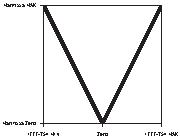
\includegraphics[width=0.97\textwidth]{Number line.pdf}}
\end{center}
\end{figure}

\begin{figure}[H]
\drawfig{fig:spirix_number_line}{Two's Complement Representation}
\begin{center}
    \fbox{\includegraphics[width=0.97\textwidth,page=2]{Number line.pdf}}
\end{center}
\end{figure}

\begin{figure}[H]
\drawfig{fig:scalar_structure}{Scalar Type Definition in Rust}
\begin{lstlisting}[style=rust]
pub struct Scalar<F: Integer, E: Integer> {
	/// The fraction component representing the significand.
	/// For normal values, any bit pattern is valid and sign bit is not included.
	/// For ambiguous values, the leading same bit count determines
	/// the state (exploded, vanished, undefined, Zero, or Infinity).
	pub fraction: F,

	/// The unsigned modular exponent determining the scale of the value.
	/// Member of cyclic group Z/2^EXP_BITS-Z; arithmetic is naturally
	/// modular at the field's native width. AMBIGUOUS_EXPONENT is the
	/// all-zeros bit pattern (the cyclic origin), reached by both
	/// overflow and underflow via opposite traversals of the cycle.
	pub exponent: E,
}
\end{lstlisting}
\end{figure}

\begin{figure}[H]
\drawfig{fig:circle_structure}{Circle Type Definition in Rust}
\begin{lstlisting}[style=rust]
pub struct Circle<F: Integer, E: Integer> {
	/// The real two's complement fraction.
	/// Leading same bit count determines state for ambiguous values.
	pub real: F,

	/// The imaginary two's complement fraction.
	/// Leading same bit count determines state for ambiguous values.
	pub imaginary: F,

	/// The shared unsigned modular exponent determining scale.
	/// Cyclic origin (all-zeros bit pattern) is AMBIGUOUS_EXPONENT.
	pub exponent: E,
}
\end{lstlisting}
\end{figure}

\begin{figure}[H]
\drawfig{fig:integer}{Where fraction: F and exponent: E are any sized integer}
\begin{lstlisting}[style=rust]
impl Integer for i8 {}
impl Integer for i16 {}
impl Integer for i32 {}
impl Integer for i64 {}
impl Integer for i128 {}
\end{lstlisting}
\end{figure}

\begin{figure}[H]
\centering
\begin{adjustbox}{angle=-90, max totalheight=0.97\textheight, max width=\textwidth}
\begin{minipage}{0.97\textheight}
\drawfig{fig:spirix_configurations}{FE Type Configurations - Precision vs. Range}
\centering
    \renewcommand{\arraystretch}{1.4}
\begin{tabular}{|c|c|c|c|c|c|}
        \hline
        \multirow{2}{*}{\textbf{Range}}  & \multicolumn{5}{c|}{\textbf{Precision (Fraction Bits) --- Scalar / Circle digits}}                                                                                                                                                          \\
        \cline{2-6}
                                         & \textbf{F3 (8-bit)}                                                                & \textbf{F4 (16-bit)}                & \textbf{F5 (32-bit)}                & \textbf{F6 (64-bit)}                & \textbf{F7 (128-bit)}                \\
                                         & 2.4 / 2.1 digits                                                           & 4.8 / 4.5 digits            & 9.6 / 9.3 digits            & 19.2 / 18.9 digits          & 38.5 / 38.2 digits           \\
        \hline
        \textbf{E3}                      & F3E3                                                                               & F4E3                                & F5E3                                & F6E3                                & F7E3                                 \\
        $\approx 10^{38.5}$      & $\langle$i8, i8$\rangle$                                                   & $\langle$i16, i8$\rangle$   & $\langle$i32, i8$\rangle$   & $\langle$i64, i8$\rangle$   & $\langle$i128, i8$\rangle$   \\
        \hline
        \textbf{E4}                      & F3E4                                                                               & F4E4                                & F5E4                                & F6E4                                & F7E4                                 \\
        $\approx 10^{9860}$      & $\langle$i8, i16$\rangle$                                                  & $\langle$i16, i16$\rangle$  & $\langle$i32, i16$\rangle$  & $\langle$i64, i16$\rangle$  & $\langle$i128, i16$\rangle$  \\
        \hline
        \textbf{E5}                      & F3E5                                                                               & F4E5                                & F5E5                                & F6E5                                & F7E5                                 \\
        $\approx 10^{10^{8.81}}$ & $\langle$i8, i32$\rangle$                                                  & $\langle$i16, i32$\rangle$  & $\langle$i32, i32$\rangle$  & $\langle$i64, i32$\rangle$  & $\langle$i128, i32$\rangle$  \\
        \hline
        \textbf{E6}                      & F3E6                                                                               & F4E6                                & F5E6                                & F6E6                                & F7E6                                 \\
        $\approx 10^{10^{18.4}}$ & $\langle$i8, i64$\rangle$                                                  & $\langle$i16, i64$\rangle$  & $\langle$i32, i64$\rangle$  & $\langle$i64, i64$\rangle$  & $\langle$i128, i64$\rangle$  \\
        \hline
        \textbf{E7}                      & F3E7                                                                               & F4E7                                & F5E7                                & F6E7                                & F7E7                                 \\
        $\approx 10^{10^{37.7}}$ & $\langle$i8, i128$\rangle$                                                 & $\langle$i16, i128$\rangle$ & $\langle$i32, i128$\rangle$ & $\langle$i64, i128$\rangle$ & $\langle$i128, i128$\rangle$ \\
        \hline
    \end{tabular}
\end{minipage}
\end{adjustbox}
\end{figure}

\begin{figure}[H]
\drawfig{fig:normalization_levels}{Stored Fraction Bit Patterns and State Classification}
\begin{center}
    \centering
    \newcommand{\varbit}[2]{%
        \node[bit, empty] (vb) at (#1, #2) {};%
        \fill[black] (vb.north east) -- (vb.south east) -- (vb.south west) -- cycle;%
    }
    \begin{adjustbox}{width=\textwidth}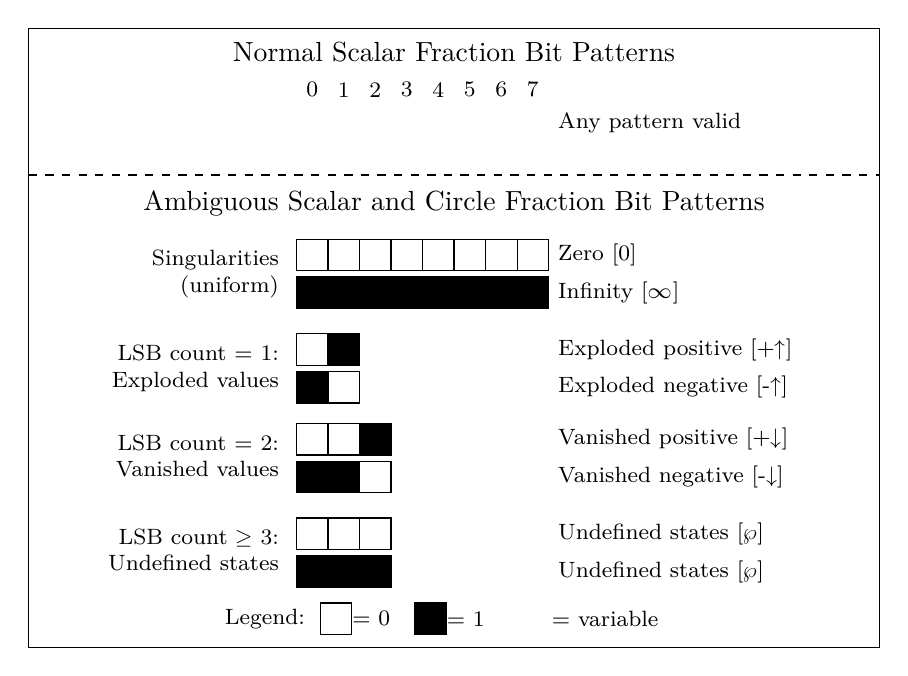
\begin{tikzpicture}[
            scale=0.6,
            every node/.style={font=\footnotesize},
            bit/.style={minimum width=0.4cm, minimum height=0.4cm, inner sep=0pt, draw, anchor=center},
            highlight/.style={fill=black},
            empty/.style={fill=white},
        ]

        % Title
        \node at (4, 10.5) {\normalsize Normal Scalar Fraction Bit Patterns};

        % Bit position markers
        \foreach \i in {0,...,7} {
                \node at (\i*0.667+1, 9.7) {\footnotesize \i};
            }

        \foreach \i in {0,...,7} {
                \varbit{\i*0.667+1}{9}
            }
        \node[align=left, anchor=west] at (6, 9) {Any pattern valid};

        % Divider
        \draw[thick, dashed] (-5, 7.9) -- (13, 7.9);
        \node[align=center] at (4, 7.3) {\normalsize{Ambiguous Scalar and Circle Fraction Bit Patterns}};

        % Zero and Infinity (uniform patterns)
        \node[align=right, anchor=east] at (0.5, 5.8) {Singularities\\(uniform)};

        % Zero pattern
        \foreach \i in {0,...,7} {
                \node[bit, empty] at (\i*0.667+1, 6.2) {};
            }
        \node[align=left, anchor=west] at (6, 6.2) {Zero [0]};

        % Infinity pattern
        \foreach \i in {0,...,7} {
                \node[bit, highlight] at (\i*0.667+1, 5.4) {};
            }
        \node[align=left, anchor=west] at (6, 5.4) {Infinity [$\infty$]};

        % LSB=1: Exploded values
        \node[align=right, anchor=east] at (0.5, 3.8) {LSB count = 1:\\Exploded values};

        % Positive exploded pattern
        \node[bit, empty] at (1, 4.2) {};
        \node[bit, highlight] at (1.667, 4.2) {};
        \foreach \i in {2,...,7} {
                \varbit{\i*0.667+1}{4.2}
            }
        \node[align=left, anchor=west] at (6, 4.2) {Exploded positive [+$\uparrow$]};

        % Negative exploded pattern
        \node[bit, highlight] at (1, 3.4) {};
        \node[bit, empty] at (1.667, 3.4) {};
        \foreach \i in {2,...,7} {
                \varbit{\i*0.667+1}{3.4}
            }
        \node[align=left, anchor=west] at (6, 3.4) {Exploded negative [-$\uparrow$]};

        % LSB=2: Vanished values
        \node[align=right, anchor=east] at (0.5, 1.95) {LSB count = 2:\\Vanished values};

        % Positive vanished pattern
        \node[bit, empty] at (1, 2.3) {};
        \node[bit, empty] at (1.667, 2.3) {};
        \node[bit, highlight] at (2.334, 2.3) {};
        \foreach \i in {3,...,7} {
                \varbit{\i*0.667+1}{2.3}
            }
        \node[align=left, anchor=west] at (6, 2.3) {Vanished positive [+$\downarrow$]};

        % Negative vanished pattern
        \node[bit, highlight] at (1, 1.5) {};
        \node[bit, highlight] at (1.667, 1.5) {};
        \node[bit, empty] at (2.334, 1.5) {};
        \foreach \i in {3,...,7} {
                \varbit{\i*0.667+1}{1.5}
            }
        \node[align=left, anchor=west] at (6, 1.5) {Vanished negative [-$\downarrow$]};

        % LSB=3+: Undefined states
        \node[align=right, anchor=east] at (0.5, -0.05) {LSB count $\geq$ 3:\\Undefined states};

        % Positive undefined patterns
        \node[bit, empty] at (1, 0.3) {};
        \node[bit, empty] at (1.667, 0.3) {};
        \node[bit, empty] at (2.334, 0.3) {};
        \foreach \i in {3,...,7} {
                \varbit{\i*0.667+1}{0.3}
            }
        \node[align=left, anchor=west] at (6, 0.3) {Undefined states [$\wp$]};

        % Negative undefined patterns
        \node[bit, highlight] at (1, -0.5) {};
        \node[bit, highlight] at (1.667, -0.5) {};
        \node[bit, highlight] at (2.334, -0.5) {};
        \foreach \i in {3,...,7} {
                \varbit{\i*0.667+1}{-0.5}
            }
        \node[align=left, anchor=west] at (6, -0.5) {Undefined states [$\wp$]};

        % Legend
        \node at (0, -1.5) {Legend:};
        \node[bit, empty] at (1.5, -1.5) {};
        \node at (2.25, -1.5) {= 0};
        \node[bit, highlight] at (3.5, -1.5) {};
        \node at (4.25, -1.5) {= 1};
        \varbit{5.5}{-1.5}
        \node at (7.2, -1.5) {= variable};

        % Border
        \draw (-5, -2.1) rectangle (13, 11);

    \end{tikzpicture}\end{adjustbox}
\end{center}
\end{figure}

\begin{figure}[H]
\drawfigA{fig:undefined}{Excerpt of Undefined State Definitions in Rust}
\begin{lstlisting}[style=rust, basicstyle=\drawmono\large]
// L3 Basic Arithmetic & Logic (leading same bit count = 3, 32 slots)
/// ¡$\square\square\square\blacksquare\blacksquare\blacksquare\blacksquare\blacksquare$¡
pub const GENERAL: Undefined = Undefined {
	prefix: 0x1F,
	symbol: "¡$\wp$¡",
	description: "General undefined or unimplemented",
};
/// ¡$\square\square\square\blacksquare\blacksquare\square\blacksquare\square$¡
pub const TRANSFINITE_PLUS_TRANSFINITE: Undefined = Undefined {
	prefix: 0x1A,
	symbol: "¡$\wp$¡¡\transfinite¡+¡\transfinite¡",
	description: "Transfinite value addition with transfinite value",
};
/// ¡$\square\square\square\blacksquare\blacksquare\square\square\square$¡
pub const NEGLIGIBLE_DIVIDE_NEGLIGIBLE: Undefined = Undefined {
	prefix: 0x18,
	symbol: "¡$\wp$¡¡\negligible¡/¡\negligible¡",
	description: "Negligible value division by negligible value",
};
\end{lstlisting}
\end{figure}

\begin{figure}[H]
\drawfigcont{B}{Excerpt of Undefined State Definitions in Rust (continued)}
\begin{lstlisting}[style=rust]
// L4 Exponentials (leading same bit count = 4, 16 slots)
/// ¡$\square\square\square\square\blacksquare\blacksquare\blacksquare\blacksquare$¡
pub const VANISHED_POWER: Undefined = Undefined {
	prefix: 0x0F,
	symbol: "¡$\wp$¡ ¡$\downarrow$¡^",
	description: "Vanished value raised to power",
};
// L5 Trigonometry (leading same bit count = 5, 8 slots)
/// ¡$\square\square\square\square\square\blacksquare\blacksquare\blacksquare$¡
pub const SINE: Undefined = Undefined {
	prefix: 0x07,
	symbol: "¡$\wp$¡ s",
	description: "Sine of value with imprecise period position",
};
// L6 Roots (leading same bit count = 6, 4 slots)
/// ¡$\square\square\square\square\square\square\blacksquare\blacksquare$¡
pub const SQRT_VANISHED: Undefined = Undefined {
	prefix: 0x03,
	symbol: "¡$\wp$¡¡$\surd$¡¡$\downarrow$¡",
	description: "Square root of vanished value",
};
\end{lstlisting}
\end{figure}

\begin{figure}[H]
\drawfig{fig:addition_table}{Addition Operation Truth Table}
\begin{center}
    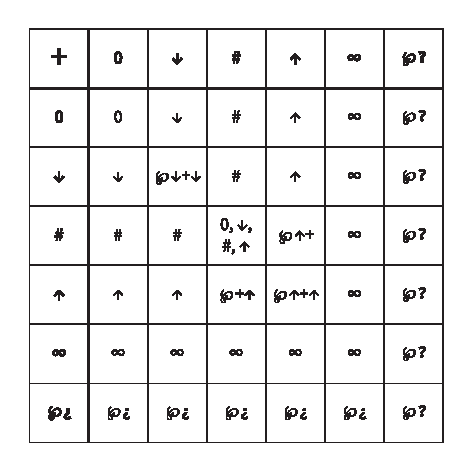
\includegraphics[width=\textwidth]{addition truth table.pdf}
\end{center}
\end{figure}

\begin{figure}[H]
\drawfig{fig:subtraction_table}{Subtraction Operation Truth Table}
\begin{center}
    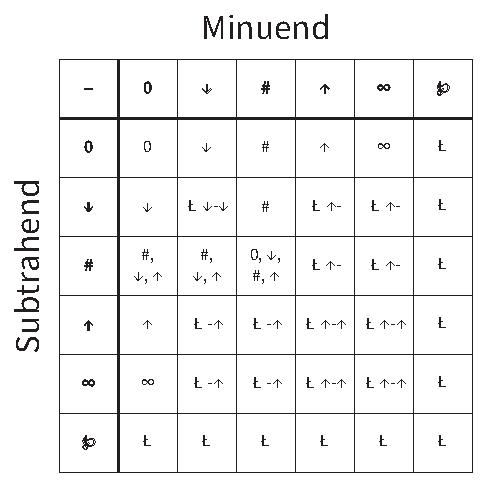
\includegraphics[width=\textwidth]{subtraction truth table.pdf}
\end{center}
\end{figure}

\begin{figure}[H]
\drawfig{fig:multiplication_table}{Multiplication Operation Truth Table}
\begin{center}
    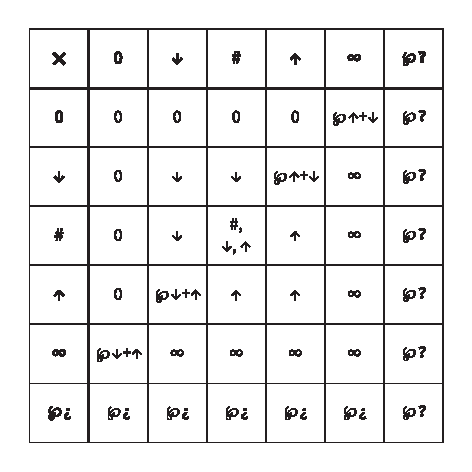
\includegraphics[width=\textwidth]{multiplication truth table.pdf}
\end{center}
\end{figure}

\begin{figure}[H]
\drawfig{fig:division_table}{Division Operation Truth Table}
\begin{center}
    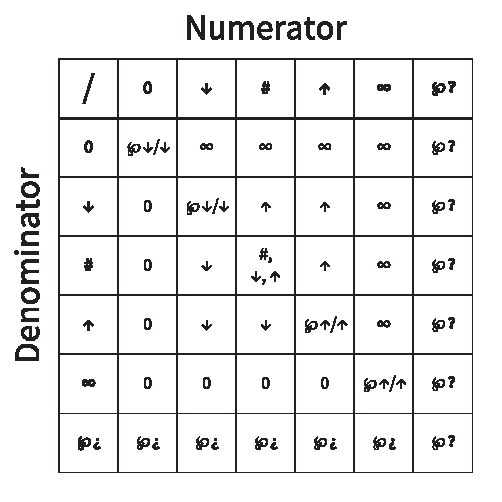
\includegraphics[width=\textwidth]{division truth table.pdf}
\end{center}
\end{figure}

\begin{figure}[H]
\drawfig{fig:spirix_ordering}{Number Line and Comparison Order}
\begin{center}
    \centering
    \begin{adjustbox}{width=\textwidth}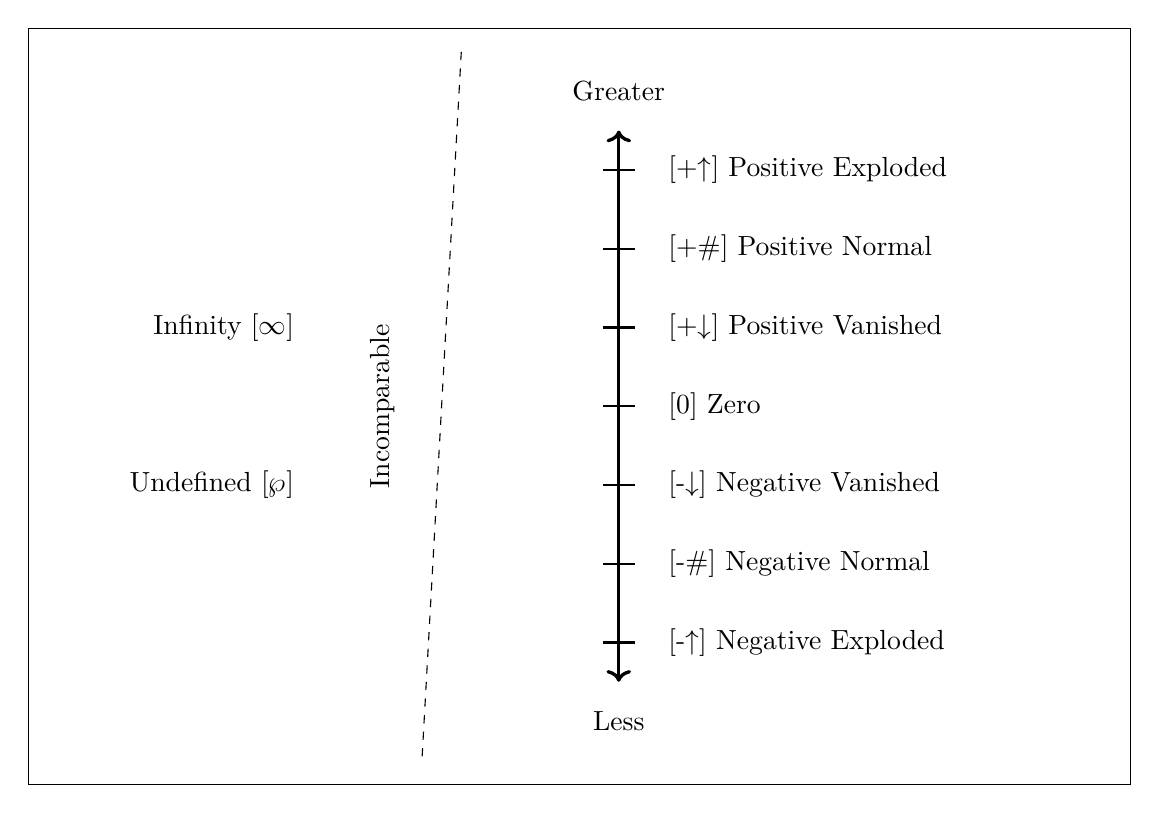
\begin{tikzpicture}[scale=1]

        \draw[<->, very thick] (0,-3.5) -- (0,3.5);
        \node[centered] at (0,4) {Greater};
        \node[centered] at (0,-4) {Less};

        \draw[thick] (-0.2,3) -- (0.2,3) node[right=0.3cm] {[+$\uparrow$] Positive Exploded};
        \draw[thick] (-0.2,2) -- (0.2,2) node[right=0.3cm] {[+\#] Positive Normal};
        \draw[thick] (-0.2,1) -- (0.2,1) node[right=0.3cm] {[+$\downarrow$] Positive Vanished};
        \draw[thick] (-0.2,0) -- (0.2,0) node[right=0.3cm] {[0] Zero};
        \draw[thick] (-0.2,-1) -- (0.2,-1) node[right=0.3cm] {[-$\downarrow$] Negative Vanished};
        \draw[thick] (-0.2,-2) -- (0.2,-2) node[right=0.3cm] {[-\#] Negative Normal};
        \draw[thick] (-0.2,-3) -- (0.2,-3) node[right=0.3cm] {[-$\uparrow$] Negative Exploded};
        \node[left] at (-4,1) {Infinity [$\infty$]};
        \node[left] at (-4,-1) {Undefined [$\wp$]};

        \draw[dashed] (-2,4.5) -- (-2.5,-4.5);
        \node[rotate=90] at (-3,0) {Incomparable};

        \draw (-7.5,-4.8) rectangle (6.5,4.8);

    \end{tikzpicture}\end{adjustbox}
\end{center}
\end{figure}

\begin{figure}[H]
\drawfigA{fig:ieee_subtract_flowchart}{IEEE 754 Binary32 Subtraction Flowchart}
\centering
\begin{adjustbox}{max width=\textwidth, max totalheight=\dimexpr\textheight-1.9\baselineskip\relax}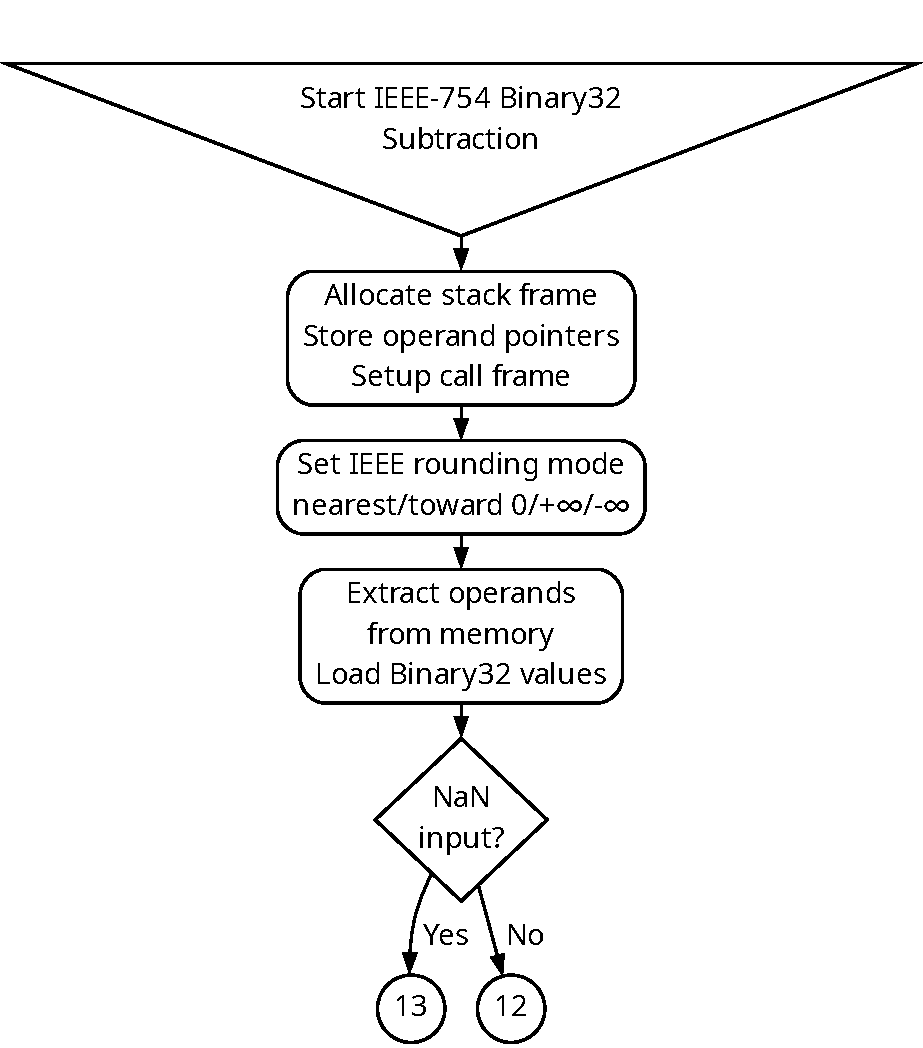
\includegraphics{flowcharts/14A.pdf}\end{adjustbox}
\end{figure}

\begin{figure}[H]
\drawfigcont{B}{IEEE 754 Binary32 Subtraction Flowchart (continued)}
\centering
\begin{adjustbox}{max width=\textwidth, max totalheight=\dimexpr\textheight-1.9\baselineskip\relax}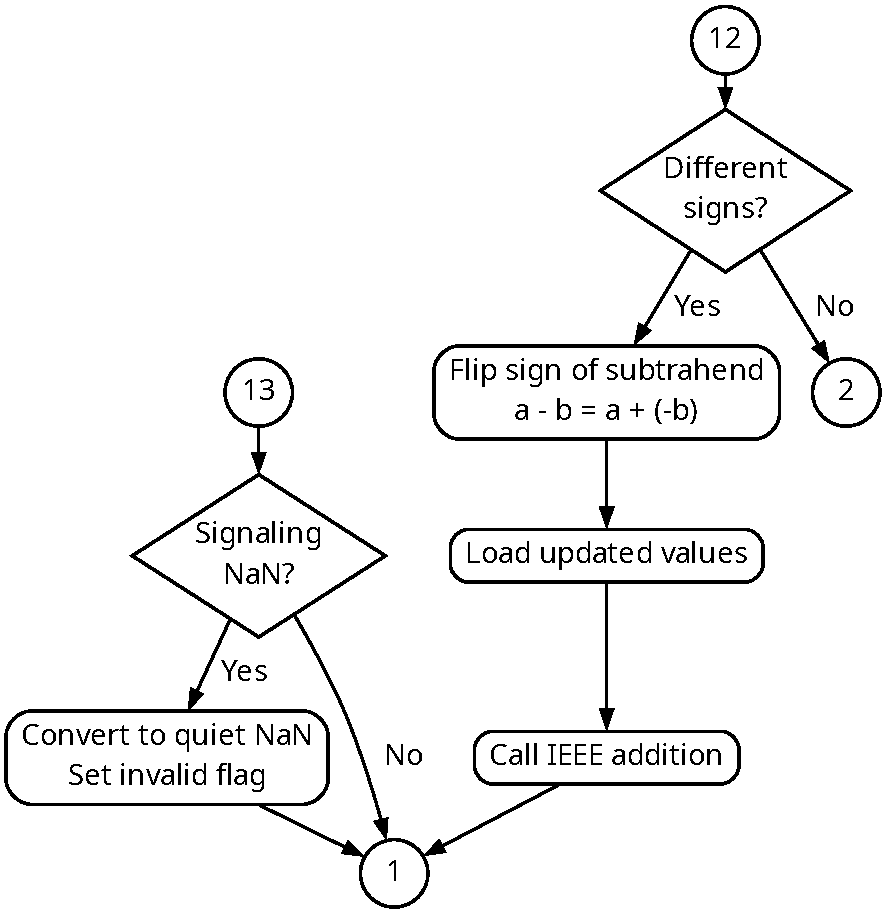
\includegraphics{flowcharts/14B.pdf}\end{adjustbox}
\end{figure}

\begin{figure}[H]
\drawfigcont{C}{IEEE 754 Binary32 Subtraction Flowchart (continued)}
\centering
\begin{adjustbox}{max width=\textwidth, max totalheight=\dimexpr\textheight-1.9\baselineskip\relax}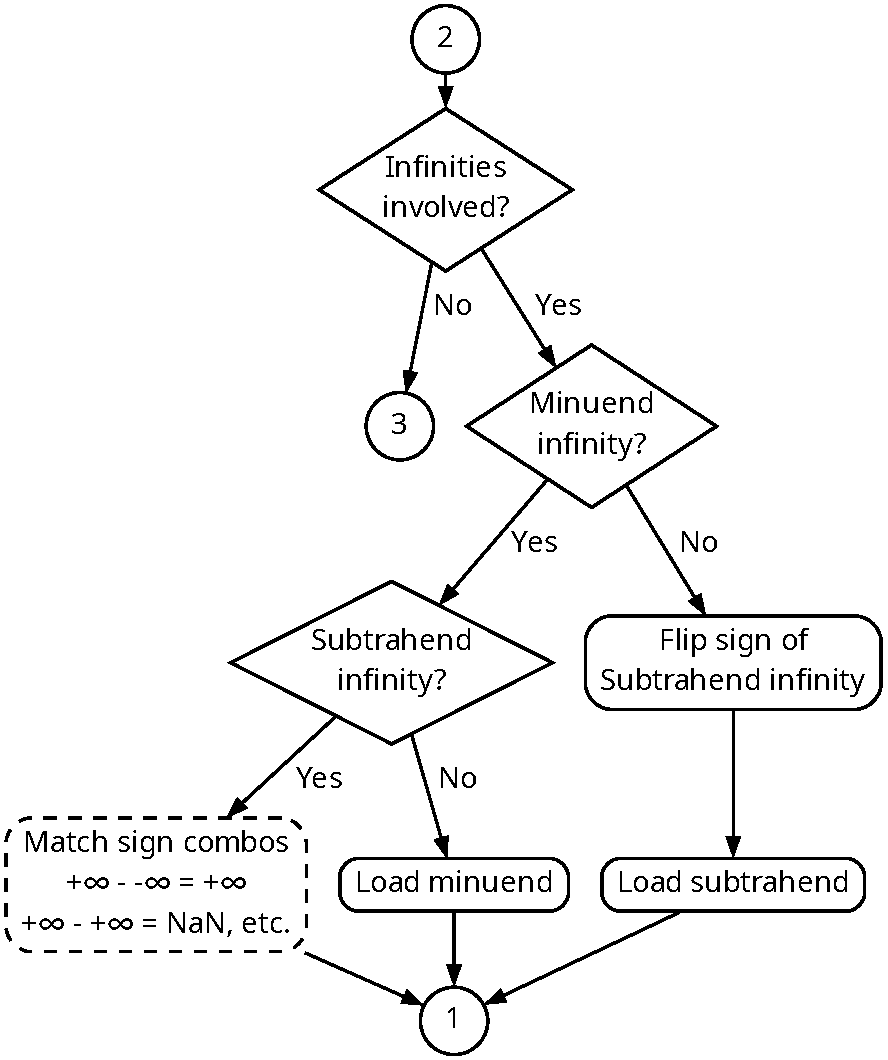
\includegraphics{flowcharts/14C.pdf}\end{adjustbox}
\end{figure}

\begin{figure}[H]
\drawfigcont{D}{IEEE 754 Binary32 Subtraction Flowchart (continued)}
\centering
\begin{adjustbox}{max width=\textwidth, max totalheight=\dimexpr\textheight-1.9\baselineskip\relax}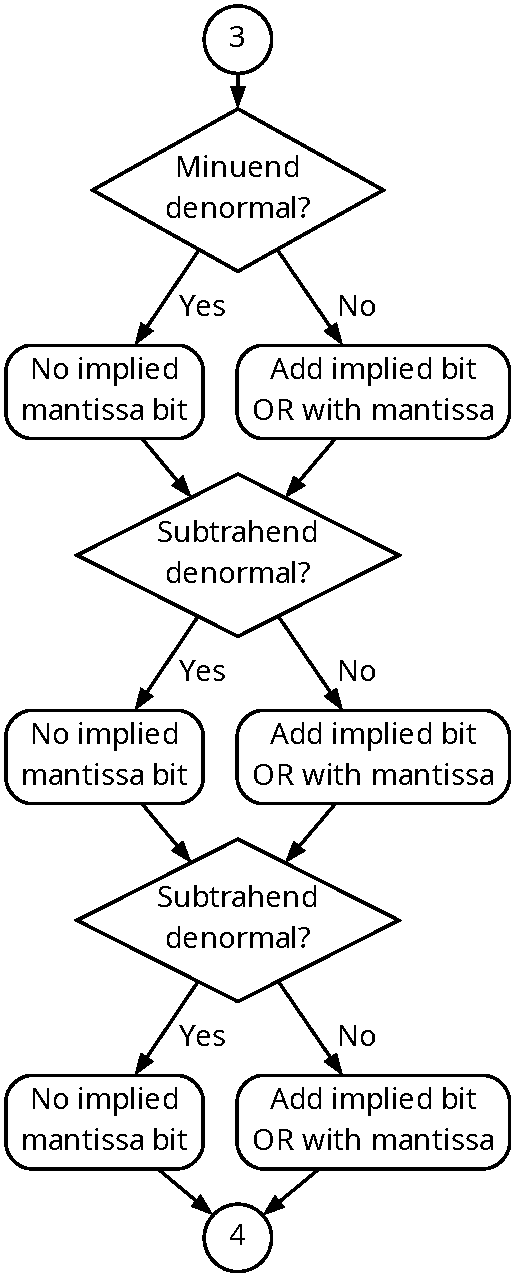
\includegraphics{flowcharts/14D.pdf}\end{adjustbox}
\end{figure}

\begin{figure}[H]
\drawfigcont{E}{IEEE 754 Binary32 Subtraction Flowchart (continued)}
\centering
\begin{adjustbox}{max width=\textwidth, max totalheight=\dimexpr\textheight-1.9\baselineskip\relax}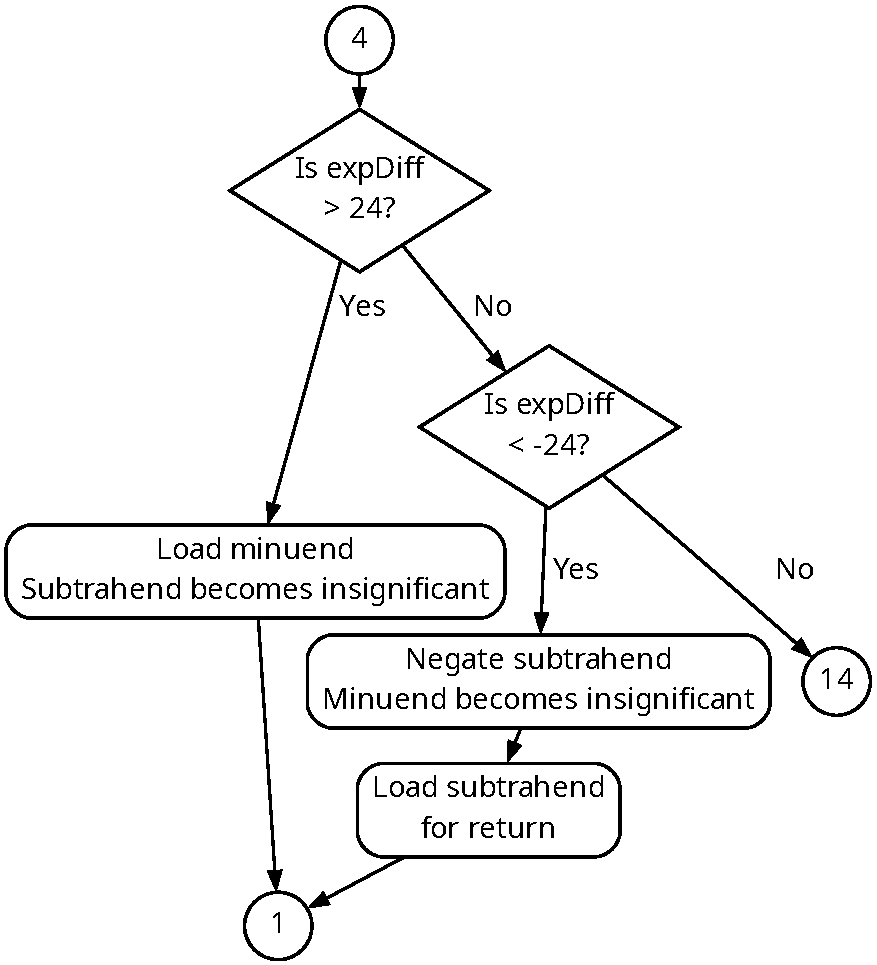
\includegraphics{flowcharts/14E.pdf}\end{adjustbox}
\end{figure}

\begin{figure}[H]
\drawfigcont{F}{IEEE 754 Binary32 Subtraction Flowchart (continued)}
\centering
\begin{adjustbox}{max width=\textwidth, max totalheight=\dimexpr\textheight-1.9\baselineskip\relax}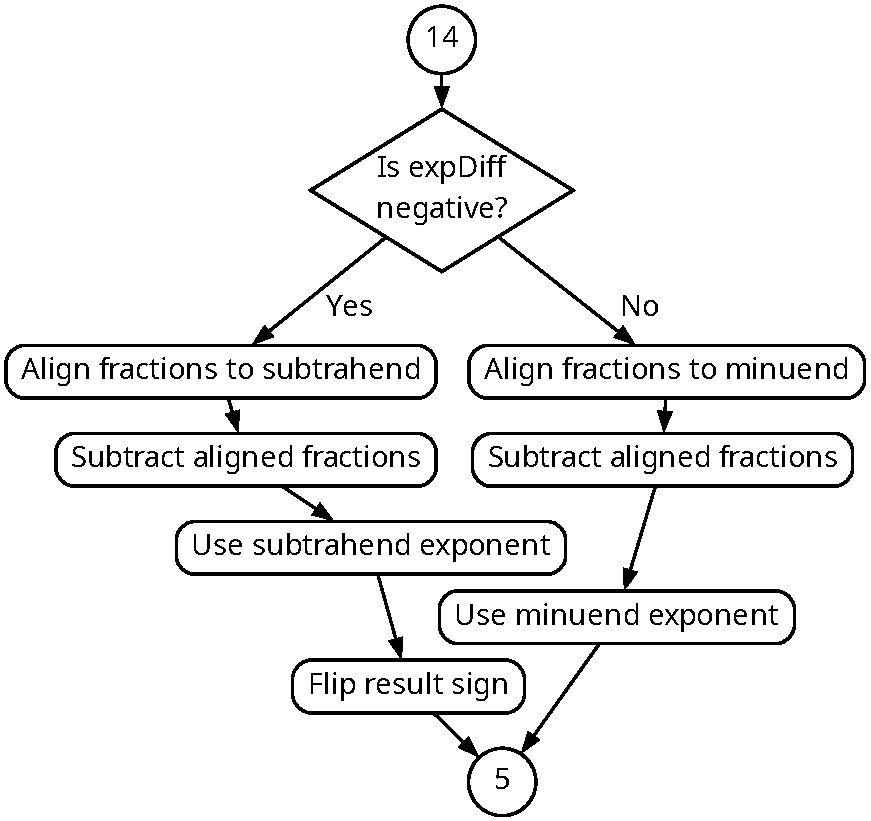
\includegraphics{flowcharts/14F.pdf}\end{adjustbox}
\end{figure}

\begin{figure}[H]
\drawfigcont{G}{IEEE 754 Binary32 Subtraction Flowchart (continued)}
\centering
\begin{adjustbox}{max width=\textwidth, max totalheight=\dimexpr\textheight-1.9\baselineskip\relax}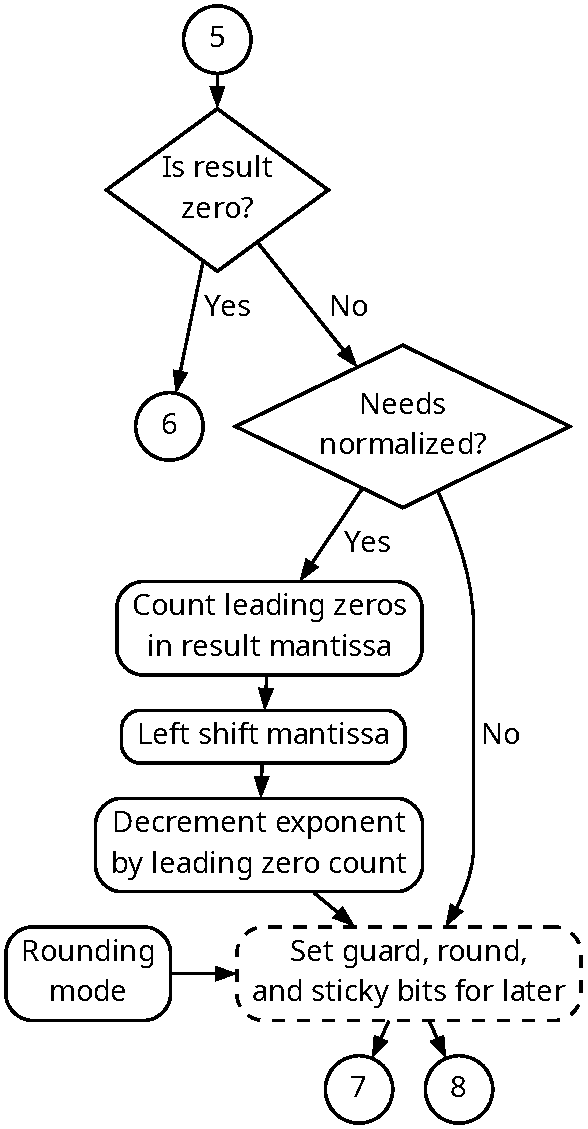
\includegraphics{flowcharts/14G.pdf}\end{adjustbox}
\end{figure}

\begin{figure}[H]
\drawfigcont{H}{IEEE 754 Binary32 Subtraction Flowchart (continued)}
\centering
\begin{adjustbox}{max width=\textwidth, max totalheight=\dimexpr\textheight-1.9\baselineskip\relax}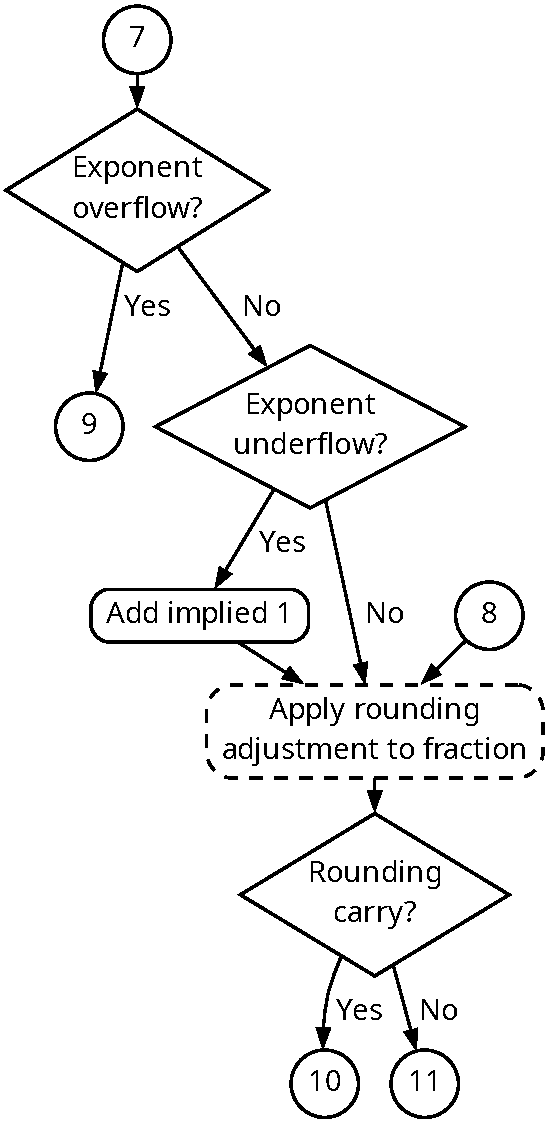
\includegraphics{flowcharts/14H.pdf}\end{adjustbox}
\end{figure}

\begin{figure}[H]
\drawfigcont{I}{IEEE 754 Binary32 Subtraction Flowchart (continued)}
\centering
\begin{adjustbox}{max width=\textwidth, max totalheight=\dimexpr\textheight-1.9\baselineskip\relax}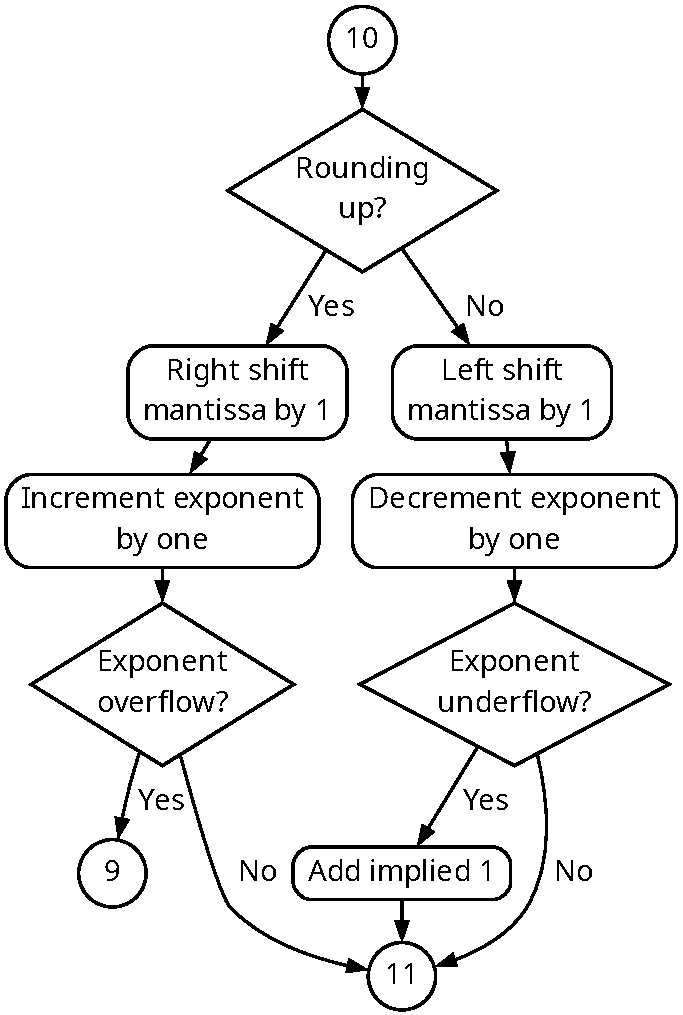
\includegraphics{flowcharts/14I.pdf}\end{adjustbox}
\end{figure}

\begin{figure}[H]
\drawfigcont{J}{IEEE 754 Binary32 Subtraction Flowchart (continued)}
\centering
\begin{adjustbox}{max width=\textwidth, max totalheight=\dimexpr\textheight-1.9\baselineskip\relax}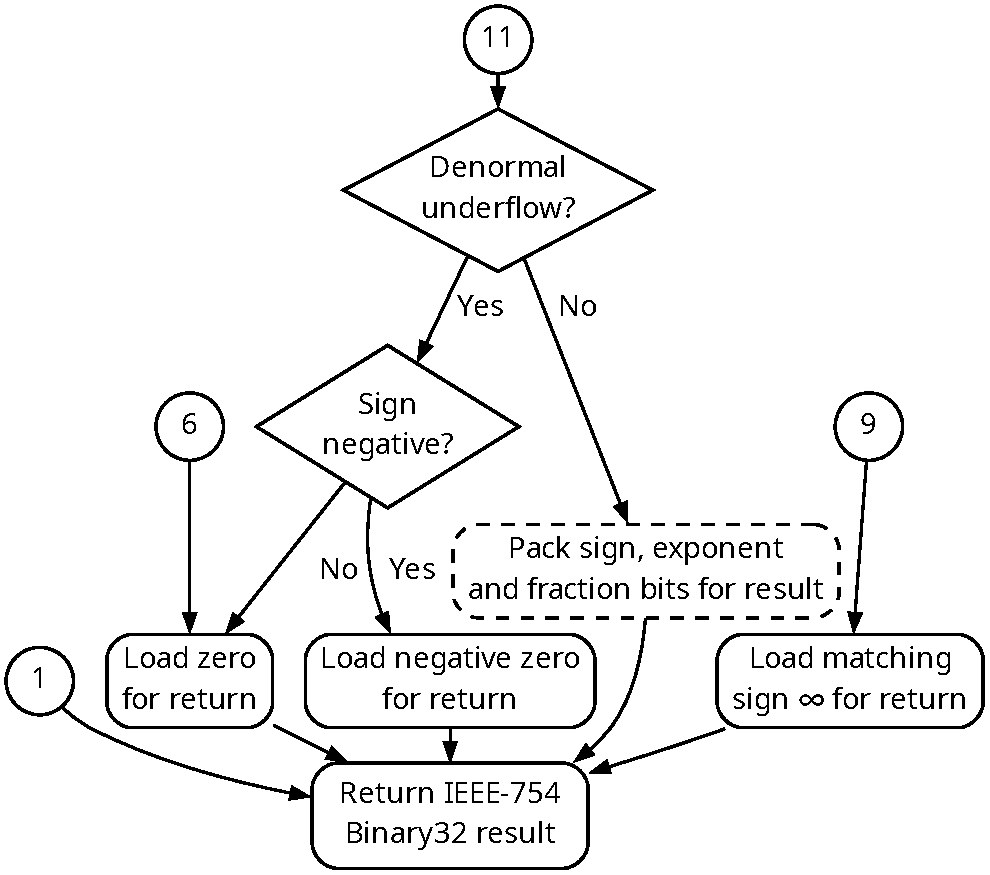
\includegraphics{flowcharts/14J.pdf}\end{adjustbox}
\end{figure}

\begin{figure}[H]
\drawfigA{fig:scalar_subtract_flowchart}{Scalar Subtraction Flowchart}
\centering
\begin{adjustbox}{max width=\textwidth, max totalheight=\dimexpr\textheight-1.9\baselineskip\relax}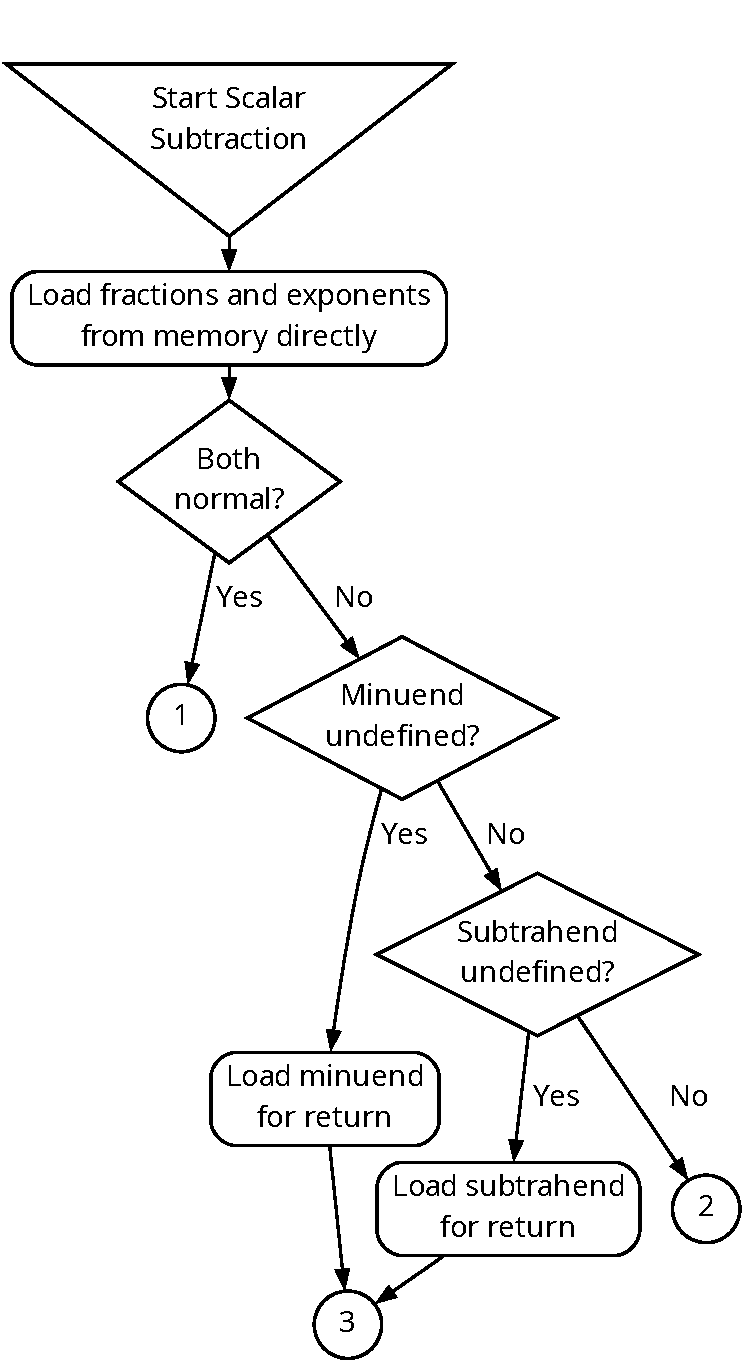
\includegraphics{flowcharts/15A.pdf}\end{adjustbox}
\end{figure}

\begin{figure}[H]
\drawfigcont{B}{Scalar Subtraction Flowchart (continued)}
\centering
\begin{adjustbox}{max width=\textwidth, max totalheight=\dimexpr\textheight-1.9\baselineskip\relax}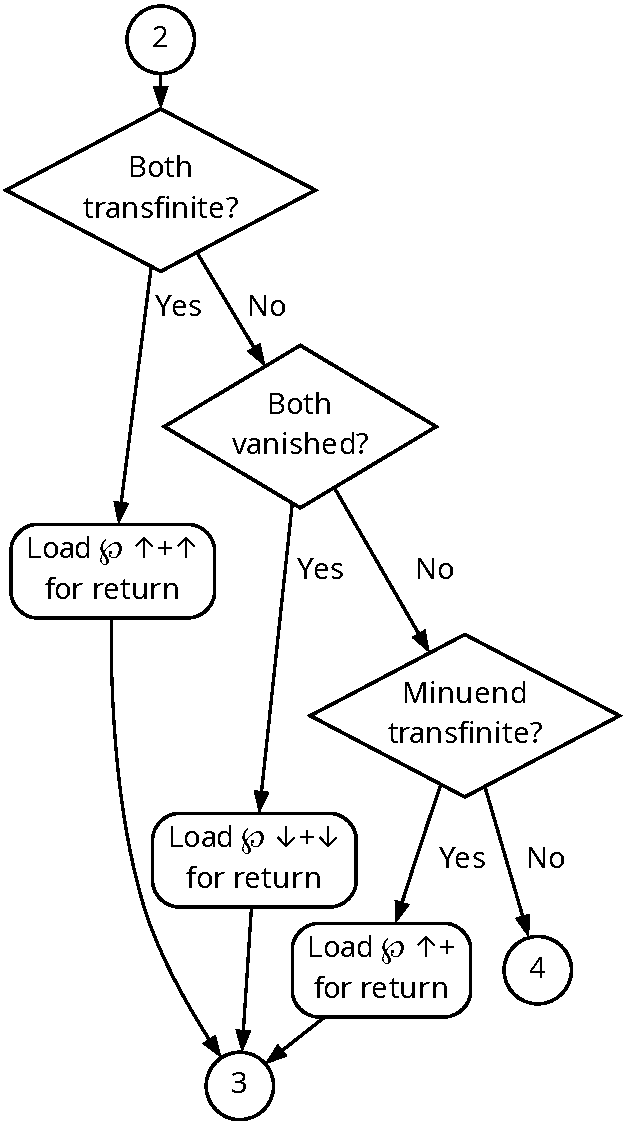
\includegraphics{flowcharts/15B.pdf}\end{adjustbox}
\end{figure}

\begin{figure}[H]
\drawfigcont{C}{Scalar Subtraction Flowchart (continued)}
\centering
\begin{adjustbox}{max width=\textwidth, max totalheight=\dimexpr\textheight-1.9\baselineskip\relax}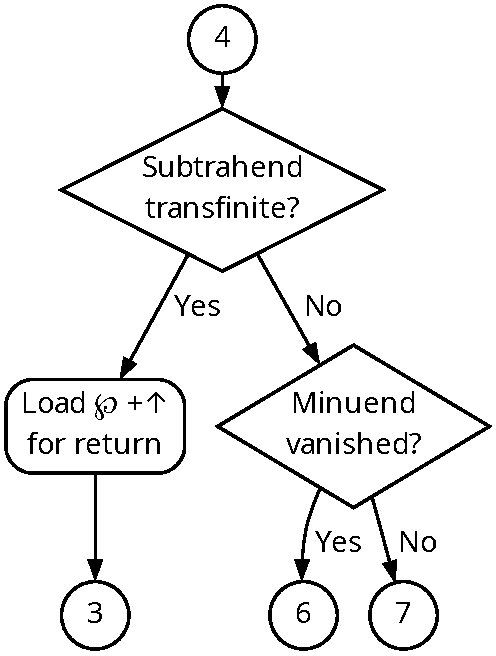
\includegraphics{flowcharts/15C.pdf}\end{adjustbox}
\end{figure}

\begin{figure}[H]
\drawfigcont{D}{Scalar Subtraction Flowchart (continued)}
\centering
\begin{adjustbox}{max width=\textwidth, max totalheight=\dimexpr\textheight-1.9\baselineskip\relax}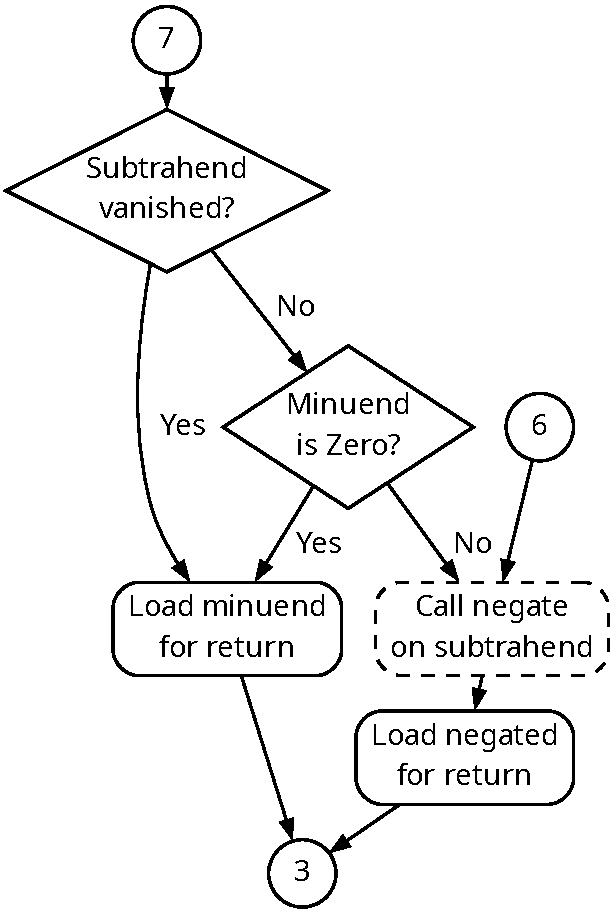
\includegraphics{flowcharts/15D.pdf}\end{adjustbox}
\end{figure}

\begin{figure}[H]
\drawfigcont{E}{Scalar Subtraction Flowchart (continued)}
\centering
\begin{adjustbox}{max width=\textwidth, max totalheight=\dimexpr\textheight-1.9\baselineskip\relax}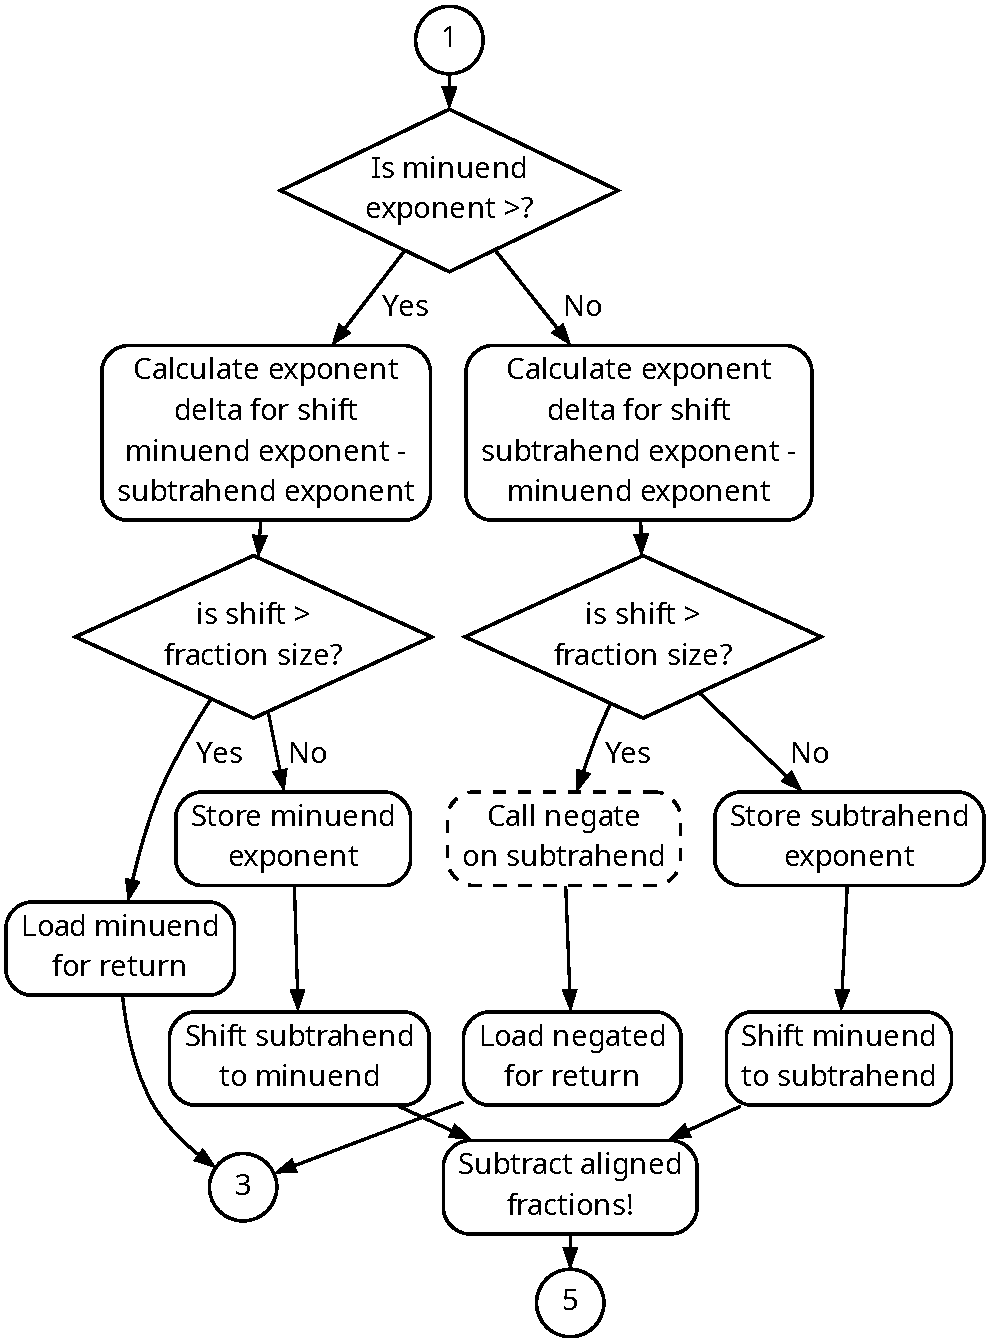
\includegraphics{flowcharts/15E.pdf}\end{adjustbox}
\end{figure}

\begin{figure}[H]
\drawfigcont{F}{Scalar Subtraction Flowchart (continued)}
\centering
\begin{adjustbox}{max width=\textwidth, max totalheight=\dimexpr\textheight-1.9\baselineskip\relax}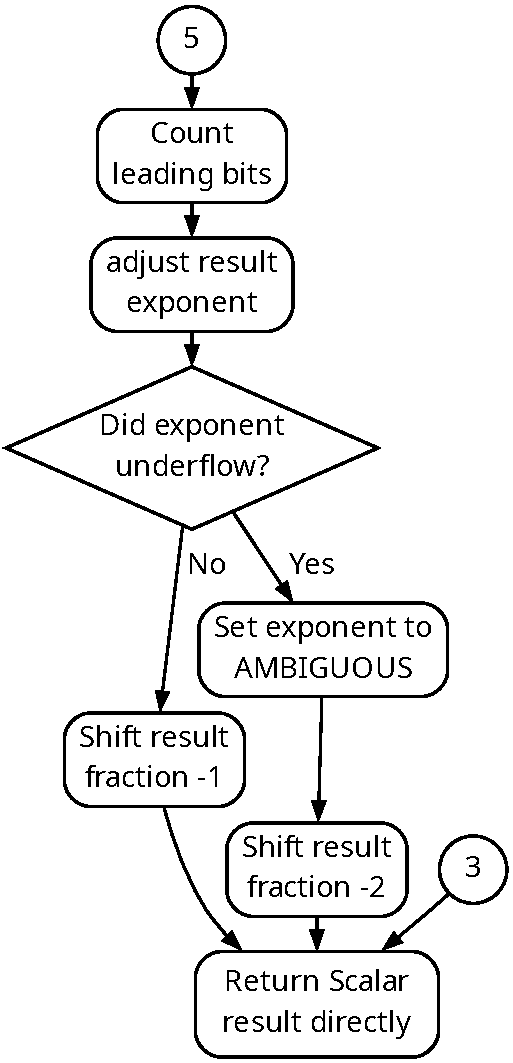
\includegraphics{flowcharts/15F.pdf}\end{adjustbox}
\end{figure}

\begin{figure}[H]
\drawfig{fig:scalar_bitwise_example}{Scalar Bitwise AND Example in Rust}
\begin{lstlisting}[style=rust]
let a = Scalar::<i32, i8>::from(42.75);  // 101010.11 in binary
let b = Scalar::<i32, i8>::from(27.5);   // 11011.1 in binary

// Bitwise AND (a & b) in the invention:
// Fractions are aligned by exponent:
//   101010.11
//    11011.1
//   ---------
//   001010.10
let result = a & b;  // Equals 10.5 in decimal, 1010.1 in binary
\end{lstlisting}
\end{figure}

\begin{figure}[H]
\drawfig{fig:scalar_bitwise_signs}{Scalar Bitwise Operations with Signs in Rust}
\begin{lstlisting}[style=rust]
// Bitwise operations respect two's complement properties
let pos = Scalar::<i32, i8>::from(42.75);   // 101010 in binary
let neg = Scalar::<i32, i8>::from(-27.5);  // ~1 00100.1 in binary
// where ~ denotes infinite leading ones

// In two's complement, negative numbers have high bits set to 1
let and_result = pos & neg;  // Will retain pos where neg has 1 bits (+32.5)
let or_result = pos | neg;   // Will be negative due to neg's high bits (-17.25)
let xor_result = pos ^ neg;  // Flips the bits of pos where neg has 1's (-49.75)
let not_result = !pos;       // Flips all bits (a smidge less than -42.75)
\end{lstlisting}
\end{figure}

\begin{figure}[H]
\drawfig{fig:scalar_shifts}{Scalar Bit Shift Operations in Rust}
\begin{lstlisting}[style=rust]
let value = Scalar::<i32, i8>::from(42);

// Left shift (multiplication by power of 2)
let shifted_left = value << 3;  // Equals 336 (42 * 2^3)

// Right shift (division by power of 2)
let shifted_right = value >> 2;  // Equals 10.5 (42 / 2^2)
\end{lstlisting}
\end{figure}

\label{LastSheet}
\end{document}
